\documentclass[14pt, a4paper]{extreport}
\usepackage[T2A]{fontenc}
\usepackage[utf8]{inputenc}
\usepackage[english, russian]{babel}
\usepackage{fontspec}
\setmainfont{Times New Roman}
\usepackage{setspace}
\setstretch{1.2857}  % 18 pt / 14 pt = 1.2857
\usepackage[top=20mm, bottom=20mm, left=30mm, right=15mm]{geometry}
\usepackage{setspace}
\onehalfspacing

\usepackage[hidelinks]{hyperref}

\usepackage{style/bsudiplomatitle}
\usepackage{style/bsumain}

\makeatletter
% Для работы с ненумерованными главами (Введение, Заключение и т.д.)
\newcommand{\unnumberedchapter}[1]{
  \chapter*{#1}
  \addcontentsline{toc}{chapter}{#1}
}

\newcommand{\ulinefill}[1]{%
  \underline{\makebox[\linewidth][l]{#1}}%
}

% Сбрасываем счетчик глав перед первым нумерованным разделом
\newcommand{\resetchaptercounter}{
  \setcounter{chapter}{0}
}

% НЕ ИСПОЛЬЗУЕМ \section - используем только \subsection как подглавы
\renewcommand{\thesubsection}{\thechapter.\arabic{subsection}}
\renewcommand{\thesubsubsection}{\thesubsection.\arabic{subsubsection}}

% Убираем нумерацию у section
\renewcommand{\thesection}{}
\setcounter{secnumdepth}{2}  % Нумеруем только до subsection
\setcounter{tocdepth}{2}     % Показываем в оглавлении до subsection

% Сбрасываем счетчики для subsection при новой главе
\let\oldchapter\chapter
\renewcommand{\chapter}{%
  \setcounter{subsection}{0}%
  \oldchapter%
}

\makeatother


\usepackage{graphicx}
\graphicspath{{images/}}

\usepackage{enumitem}
\setlist{nosep, leftmargin=*}

\usepackage{tabularx}
\usepackage{booktabs}
\usepackage{caption}
\captionsetup[table]{justification=raggedright, singlelinecheck=false, font=small, labelfont=bf}
\captionsetup[figure]{justification=centering, font=small, labelfont=bf}

\usepackage{listings}
\usepackage{xcolor}
\lstset{
    basicstyle=\ttfamily\small,
    breaklines=true,
    frame=single,
    numbers=left,
    numberstyle=\tiny\color{gray},
    tabsize=4,
    inputencoding=utf8,
    extendedchars=true
}

\usepackage{fancyhdr}
\pagestyle{fancy}
\fancyhf{}
\fancyfoot[C]{\thepage}
\renewcommand{\headrulewidth}{0pt}

\usepackage{float}
\usepackage{wrapfig}

\title{ОЦЕНКА КАЧЕСТВА ЭНТРОПИИ В БИОЛОГИЧЕСКИХ ГЕНЕРАТОРАХ СЛУЧАЙНЫХ ЧИСЕЛ НА ОСНОВЕ ПОВЕДЕНЧЕСКИХ ФАКТОРОВ}
\author{САЗОНЧИК Иван Михайлович}
\mentor{старший преподаватель М.А. Казловский}
\subfaculty{}   % оставляем пустым, т.к. шапка уже содержит кафедру
\reviewer{Заведующий кафедрой математического\\ 
          моделирования и анализа данных\\
          доктор экономических наук, кандидат физико-\\
          математических наук, профессор В.И. Малюгин}

\begin{document}
\maketitle
% ===== ЗАДАНИЕ НА ДИПЛОМНУЮ РАБОТУ =====
\newpage
\thispagestyle{empty}
\begin{center}
\textbf{Белорусский государственный университет}
 
Кафедра математического моделирования и анализа данных
\end{center}
 
\vspace{1cm}
 
\begin{flushright}
\textbf{УТВЕРЖДАЮ}\\
Заведующий \underline{\hspace{3cm}} кафедрой\\[0.5cm]
\underline{\hspace{4cm}}\\
{\footnotesize (подпись) (фамилия, инициалы)}\\[0.3cm]
\underline{\hspace{1.5cm}} \underline{\hspace{3cm}} 20\underline{\hspace{0.5cm}} г.
\end{flushright}
 
\vspace{1.5cm}
 
\begin{center}
\textbf{ЗАДАНИЕ НА ДИПЛОМНУЮ РАБОТУ}
\end{center}
 
\vspace{1cm}
 
\noindent Обучающемуся \underline{Сазончику Ивану Михайловичу}\\
{\centering\footnotesize (фамилия, собственное имя, отчество (если таковое имеется))\par}
 
\noindent Курс \underline{\hspace{2.5cm}4\hspace{2.5cm}} \quad Учебная группа \underline{\hspace{2.5cm}9\hspace{2.5cm}}
 
\noindent Специальность \underline{\hspace{3cm}компьютерная безопасность\hspace{3cm}}
 
\vspace{0.8cm}
 
\noindent Тема дипломной работы \underline{\makebox[\dimexpr\linewidth-6.2cm][l]{ Оценка качества энтропии в биологических}}
\noindent\underline{\makebox[\linewidth][l]{генераторах случайных чисел на основе поведенческих факторов}}
{\centering\footnotesize (наименование темы)\par}
 
\vspace{0.5cm}
 
\noindent Утверждена приказом ректора БГУ от \underline{\hspace{2.5cm}} №\underline{\hspace{2.5cm}}
 
\vspace{0.8cm}
 
\noindent Исходные данные к дипломной работе \\
\noindent\underline{\makebox[\linewidth][l]{1. Rukhin A. et al. A Statistical Test Suite for Random and Pseudorandom Number}}
\noindent\underline{\makebox[\linewidth][l]{Generators for Cryptographic Applications.}}
\noindent\underline{\makebox[\linewidth][l]{ NIST Special Publication 800-22. --2010. -- 131~с.}}
 
\noindent\underline{\makebox[\linewidth][l]{2.  Агиевич, С. В. Криптографические методы / С. В. Агиевич//НИИ прикладных }}
\noindent\underline{\makebox[\linewidth][l]{проблем математики и информатики БГУ.}}

\noindent\underline{\makebox[\linewidth][l]{3. Ямпольский, В. В. Биометрические методы и средства идентификации }}
\noindent\underline{\makebox[\linewidth][l]{личности/ В. В. Ямпольский, Д. В. Михеев. — М.}}
\newpage
\thispagestyle{empty}
\noindent\underline{\makebox[\linewidth][l]{: Горячая линия–Телеком, 2011. — 312 с}}
\vspace{0.8cm}
 
\noindent Перечень подлежащих разработке вопросов или краткое содержание расчётно-пояснительной записки:
 
\noindent\underline{\makebox[\linewidth][l]{1. Подготовить обзор научной литературы, определить цели и задачи}}
\noindent\underline{\makebox[\linewidth][l]{исследования.}}
\noindent\underline{\makebox[\linewidth][l]{2. Разработать программный комплекс для захвата и обработки окуломоторных}}
\noindent\underline{\makebox[\linewidth][l]{и голосовых данных.}}

\noindent\underline{\makebox[\linewidth][l]{3. Реализовать алгоритмы извлечения, накопления и смешивания энтропии}}
\noindent\underline{\makebox[\linewidth][l]{из двух каналов.}}

\noindent\underline{\makebox[\linewidth][l]{4. Реализовать оценку статистического качества генерируемых }}
\noindent\underline{\makebox[\linewidth][l]{последовательностей (NIST SP~800-90B).}}

\noindent\underline{\makebox[\linewidth][l]{5. Провести компьютерный эксперимент и анализ результатов.}}
 
\vspace{0.5cm}
 
\noindent Перечень графического материала (с точным указанием обязательных чертежей и графиков)
 
\noindent\underline{\hspace{\textwidth}}
 
\noindent\underline{\hspace{\textwidth}}
 
\vspace{0.5cm}
 
\noindent Консультанты по дипломной работе (с указанием разделов, по которым они консультируют)\underline{\hspace{3cm}}
 
\noindent\underline{\hspace{\textwidth}}
 
\vspace{0.5cm}
 
\noindent Примерный календарный график выполнения дипломной работы
 
\noindent\underline{\hspace{\textwidth}}
 
\noindent\underline{\hspace{\textwidth}}
 
\noindent\underline{\hspace{\textwidth}}
 
\vspace{0.3cm}
 
\noindent Дата выдачи задания\underline{\hspace{6cm}}
 
\noindent Сроки сдачи законченной дипломной работы\underline{\hspace{4cm}}
 
\vspace{0.5cm}
 
\noindent Руководитель дипломной работы \underline{\hspace{2cm}} \underline{\hspace{3cm}}\\
{\hspace{5.5cm}\footnotesize (подпись) \hspace{2cm} (инициалы, фамилия)\par}
 
\noindent Подпись обучающегося \underline{\hspace{6cm}}
 
\noindent Дата\underline{\hspace{3cm}} 20\underline{\hspace{0.5cm}} г.
 
\vspace{1.5cm}
\newpage
\thispagestyle{empty}
\noindent Проинформирован о недопустимости привлечения третьих лиц к выполнению дипломной работы, плагиата, фальсификации или подлога материалов.
 
\vspace{0.8cm}
 
\noindent\underline{\hspace{3cm}} \quad \underline{\hspace{5cm}}\\
{\hspace{1cm}\footnotesize (подпись) \hspace{1.5cm} (инициалы, фамилия)\par}
% ===== КОНЕЦ ЗАДАНИЯ =====
\pagenumbering{arabic} % Включаем арабскую нумерацию
\setcounter{page}{1}   % Устанавливаем начальное значение = 3
\renewcommand{\contentsname}{\centering ОГЛАВЛЕНИЕ}
\tableofcontents
\newpage
\begin{center}{\bf \Large Реферат}\end{center}
 
\textbf{Дипломная работа:} 43 страницы, 4 рисунка, 2 таблицы, 4 источника, 3 приложения.
 
\textbf{Ключевые слова:} БИОЛОГИЧЕСКИЙ ГЕНЕРАТОР СЛУЧАЙНЫХ ЧИСЕЛ, ЭНТРОПИЯ,
ДВИЖЕНИЯ ГЛАЗ, ГОЛОСОВОЙ СИГНАЛ, ОКУЛОМОТОРНАЯ АКТИВНОСТЬ, НЕЙРОМЫШЕЧНАЯ
НЕСТАБИЛЬНОСТЬ, МЕЛ-КЕПСТРАЛЬНЫЕ КОЭФФИЦИЕНТЫ, СТАТИСТИЧЕСКОЕ ТЕСТИРОВАНИЕ,
NIST SP~800-90B, КРИПТОГРАФИЧЕСКИЙ КЛЮЧ.
 
\textbf{Объект исследования:} энтропия, извлекаемая из поведенческих
биометрических сигналов человека -- траектории движения глаз и голоса.
 
\textbf{Цель работы:} разработка, программная реализация и комплексная оценка
качества биологического генератора случайных чисел, использующего два
поведенческих биометрических канала -- движения глаз и голос человека --
в качестве источников энтропии для формирования криптографических ключей.
 
\textbf{Методы исследования:}
 
а) теоретические: изучение источников, посвящённых классификации генераторов
случайных чисел и источников энтропии согласно стандарту СТБ~34.101.27-2022;
анализ биофизических основ окуломоторной активности и голосообразования как
источников непредсказуемости; изучение методологии оценки энтропии
NIST SP~800-90B;
 
б) практические: разработка программного комплекса на языке Python с
применением библиотек MediaPipe и OpenCV для захвата и обработки движений
глаз; реализация модуля сбора голосовой энтропии на основе анализа
амплитудных, спектральных и темпоральных характеристик акустического сигнала;
статистическое тестирование генерируемых последовательностей с использованием
утилит \texttt{ea\_iid} и \texttt{ea\_non\_iid} пакета NIST SP~800-90B;
экспериментальное исследование влияния типа активности пользователя на
качество извлекаемой энтропии.
 
\textbf{Результат:} разработан и реализован программный комплекс для генерации
криптографических ключей длиной 128 и 256 бит на основе двух биометрических
каналов; реализованы алгоритмы квантования и бит-экстракции для движений глаз
и голосового сигнала; разработан механизм смешивания энтропии через
конкатенацию с последующим хешированием SHA-256; проведено
экспериментальное исследование с участием 12 добровольцев в четырёх сценариях
активности; установлено, что наилучшие показатели энтропии (7{,}3--7{,}5
бит/байт) достигаются при свободной речи и просмотре динамичного видео;
генерируемые последовательности успешно проходят тесты NIST SP~800-90B.
 
\textbf{Область применения:} проектирование программных генераторов случайных
чисел с истинной энтропией для использования в криптографических системах
защиты информации.
 
 
 
\newpage
\begin{center}{\bf \Large Рэферат}\end{center}
 
\textbf{Дыпломная праца:} 43 старонкі, 4 малюнка, 2 табліцы, 4 крыніцы, 3 дадатка.
 
\textbf{Ключавыя словы:} БІЯЛАГІЧНЫ ГЕНЕРАТАР ВЫПАДКОВЫХ ЛІКАЎ, ЭНТРАПІЯ,
РУХ ВАЧЭЙ, ГАЛАСАВЫ СІГНАЛ, АКУЛАМАТОРНАЯ АКТЫЎНАСЦЬ, НЕЙРАМЫШАЧНАЯ
НЕСТАБІЛЬНАСЦЬ, МЕЛ-КЕПСТРАЛЬНЫЯ КАЭФІЦЫЕНТЫ, СТАТЫСТЫЧНАЕ ТЭСТАВАННЕ,
NIST SP~800-90B, КРЫПТАГРАФІЧНЫ КЛЮЧ.
 
\textbf{Аб'ект даследавання:} энтрапія, якая здабываецца з паводзінавых
біяметрычных сігналаў чалавека -- траекторыі руху вачэй і голасу.
 
\textbf{Мэта работы:} распрацоўка, праграмная рэалізацыя і комплексная ацэнка
якасці біялагічнага генератара выпадковых лікаў, які выкарыстоўвае два
паводзінавых біяметрычных канала -- рух вачэй і голас чалавека -- у якасці
крыніц энтрапіі для фарміравання крыптаграфічных ключоў.
 
\textbf{Метады даследавання:}
 
а) тэарэтычныя: вывучэнне крыніц, прысвечаных класіфікацыі генератараў
выпадковых лікаў і крыніц энтрапіі згодна са стандартам СТБ~34.101.27-2022;
аналіз біяфізічных асноў акуламаторнай актыўнасці і галасаўтварэння як
крыніц непрадказальнасці; вывучэнне метадалогіі ацэнкі энтрапіі
NIST SP~800-90B;
 
б) практычныя: распрацоўка праграмнага комплексу на мове Python з
выкарыстаннем бібліятэк MediaPipe і OpenCV для захопу і апрацоўкі руху вачэй;
рэалізацыя модуля збору галасавой энтрапіі на аснове аналізу амплітудных,
спектральных і тэмпаральных характарыстык акустычнага сігналу; статыстычнае
тэставанне генераваных паслядоўнасцей з дапамогай утыліт \texttt{ea\_iid}
і \texttt{ea\_non\_iid} пакета NIST SP~800-90B; эксперыментальнае даследаванне
ўплыву тыпу актыўнасці карыстальніка на якасць здабываемай энтрапіі.
 
\textbf{Вынік:} распрацаваны і рэалізаваны праграмны комплекс для генерацыі
крыптаграфічных ключоў даўжынёй 128 і 256 біт на аснове двух біяметрычных
каналаў; рэалізаваны алгарытмы квантавання і біт-экстракцыі для руху вачэй
і галасавога сігналу; распрацаваны механізм змешвання энтрапіі праз
канкатэнацыю з наступным хэшаваннем SHA-256; праведзена эксперыментальнае
даследаванне з удзелам 12 добраахвотнікаў у чатырох сцэнарыях актыўнасці;
устаноўлена, што найлепшыя паказчыкі энтрапіі (7{,}3--7{,}5 біт/байт)
дасягаюцца пры свабоднай мове і праглядзе дынамічнага відэа; генераваныя
паслядоўнасці паспяхова праходзяць тэсты NIST SP~800-90B.
 
\textbf{Вобласць ужывання:} праектаванне праграмных генератараў выпадковых
лікаў з сапраўднай энтрапіяй для выкарыстання ў крыптаграфічных сістэмах
абароны інфармацыі.
 
 
 
\newpage
\begin{center}{\bf \Large Abstract}\end{center}
 
\textbf{Diploma thesis:} 43 pages, 4 images, 2 tables, 4 sources, 3 appendices.
 
\textbf{Keywords:} BIOLOGICAL RANDOM NUMBER GENERATOR, ENTROPY, EYE
MOVEMENTS, VOICE SIGNAL, OCULOMOTOR ACTIVITY, NEUROMUSCULAR INSTABILITY,
MEL-FREQUENCY CEPSTRAL COEFFICIENTS, STATISTICAL TESTING, NIST SP~800-90B,
CRYPTOGRAPHIC KEY.
 
\textbf{The object of the study:} entropy extracted from human behavioural
biometric signals -- eye movement trajectories and voice.
 
\textbf{The purpose of the work:} development, software implementation and
comprehensive quality assessment of a biological random number generator that
uses two behavioural biometric channels -- eye movements and human voice --
as entropy sources for cryptographic key generation.
 
\textbf{Research methods:}
 
a) theoretical: study of sources devoted to the classification of random
number generators and entropy sources in accordance with the standard
STB~34.101.27-2022; analysis of the biophysical foundations of oculomotor
activity and voice production as sources of unpredictability; study of the
NIST SP~800-90B entropy assessment methodology;
 
b) practical: development of a software suite in Python using the MediaPipe
and OpenCV libraries for capturing and processing eye movements; implementation
of a voice entropy collection module based on the analysis of amplitude,
spectral and temporal characteristics of the acoustic signal; statistical
testing of generated sequences using the \texttt{ea\_iid} and
\texttt{ea\_non\_iid} utilities from the NIST SP~800-90B package;
experimental investigation of the influence of user activity type on the
quality of extracted entropy.
 
\textbf{Result:} a software suite for generating cryptographic keys of 128
and 256 bits based on two biometric channels has been developed and
implemented; quantisation and bit-extraction algorithms for eye movements and
voice signal have been realised; an entropy mixing mechanism via concatenation followed by SHA-256 hashing has been developed; an
experimental study involving 12 volunteers across four activity scenarios has
been conducted; it has been established that the best entropy values
(7.3--7.5 bits/byte) are achieved during free speech and dynamic video
viewing; the generated sequences successfully pass the NIST SP~800-90B tests.
 
\textbf{Scope:} design of software true-entropy random number generators for
use in cryptographic information protection systems.
\newpage
\unnumberedchapter{ВВЕДЕНИЕ}

В современных условиях цифровой трансформации и повсеместного внедрения криптографических систем надёжная генерация случайных чисел является фундаментальной задачей информационной безопасности. Случайные числа и ключевые последовательности используются в широком спектре приложений: от шифрования данных и цифровых подписей до протоколов аутентификации и лотерейных систем. Качество таких последовательностей напрямую определяет устойчивость криптосистем к атакам.

Традиционные генераторы случайных чисел (ГСЧ) можно разделить на три основных класса: алгоритмические (псевдослучайные), физические (аппаратные) и комбинированные. Алгоритмические ГСЧ, хотя и обладают высокой скоростью и воспроизводимостью, по своей природе детерминированы и уязвимы при компрометации начального состояния (seed). Физические ГСЧ, основанные на измерениях шумовых процессов (тепловой шум, радиоактивный распад и др.), обеспечивают истинную случайность, но часто требуют специализированного и дорогостоящего оборудования, а их выход может быть подвержен нестабильности и внешним помехам. Всё это актуализирует поиск новых, доступных, недетерминированных и устойчивых источников энтропии, интегрируемых в повседневные вычислительные среды.

Перспективным направлением в этой области является использование биометрических данных человека. Биометрия, изучающая уникальные физиологические и поведенческие характеристики индивидов, предлагает два основных типа источников энтропии [4]. К \textit{физиологическим} относятся относительно стабильные во времени, но сложные для непрерывного измерения параметры, такие как ритмы сердца (ЭКГ), мозговые волны (ЭЭГ), характеристика кровотока. \textit{Поведенческие} факторы, напротив, отражают динамические и зачастую непредсказуемые паттерны деятельности человека: динамика нажатий клавиш, движения компьютерной мыши, жесты, речь и саккадические движения глаз.

Особый интерес представляют два взаимодополняющих поведенческих канала: окуломоторная активность и голос. Движения глаз даже при фиксации на статичном объекте демонстрируют микродвижения (тремор, дрейф, микросаккады), которые являются принципиально непредсказуемыми. Голосовой сигнал, в свою очередь, содержит несколько независимых источников случайности: нейромышечную нестабильность (джиттер, шиммер), турбулентность воздушного потока при произнесении щелевых согласных, тепловой шум аналогово-цифрового преобразователя и микровариации артикуляции. Оба канала не требуют специализированного оборудования: достаточно стандартной веб-камеры и микрофона. Их совместное использование позволяет не только увеличить скорость генерации энтропии, но и обеспечить устойчивость к компрометации одного из источников.

\textbf{Целью данной работы} является разработка, программная реализация и комплексная оценка качества биологического генератора случайных чисел, использующего два поведенческих фактора -- траекторию движения глаз и голос человека.

Для достижения поставленной цели в ходе исследования были последовательно решены следующие \textbf{задачи}:
\begin{enumerate}
\item Разработка программного комплекса для захвата видеопотока с веб-камеры, трекинга лицевых ориентиров и выделения параметров движения глаз (координаты взгляда, скорость, направление, состояние век) в реальном времени.
\item Реализация модуля сбора голосовой энтропии, работающего асинхронно и извлекающего случайность из амплитудных, спектральных и темпоральных характеристик акустического сигнала.
\item Разработка алгоритмов извлечения и накопления энтропии из двух каналов, включающих фильтрацию артефактов (закрытые глаза, тишина), квантование параметров и формирование битовой последовательности.
\item Реализация механизма смешивания энтропии из двух источников через XOR-конкатенацию с последующим хэшированием SHA-256 для получения криптографически стойкого ключа.
\item Оценка статистического качества и непредсказуемости генерируемых битовых последовательностей с использованием набора стандартизированных методов оценки NIST SP 800-90B.
\item Экспериментальное исследование влияния контекста деятельности пользователя (произвольные движения глаз, просмотр видео, свободная речь, чтение вслух) на количественные и качественные характеристики извлекаемой энтропии из каждого канала в отдельности и из их комбинации.
\end{enumerate}

\textbf{Объектом исследования} выступает энтропия, извлекаемая из поведенческих биометрических сигналов человека -- траектории движения глаз и голоса.

\textbf{Предметом исследования} являются алгоритмы и методы извлечения, обработки, смешивания и статистической оценки энтропии из данных трекинга взгляда и акустического сигнала.

Практическая значимость работы заключается в демонстрации возможности построения доступного программного ГСЧ с истинной энтропией, использующего стандартные аппаратные средства (веб-камеру и микрофон), а также в создании готового инструментария для генерации криптографических ключей. Теоретическая ценность состоит в исследовании свойств энтропии, порождаемой двумя различными биологическими системами (окуломоторной и фонаторной), и влиянии на эти свойства внешнего когнитивного контекста.

\newpage
\resetchaptercounter  % Сбросить счетчик глав
\chapter{ТЕОРЕТИЧЕСКИЕ ОСНОВЫ БИОЛОГИЧЕСКИХ ГЕНЕРАТОРОВ СЛУЧАЙНЫХ ЧИСЕЛ}

\subsection{Классификация источников энтропии}

В соответствии со стандартом СТБ 34.101.27-2022 «Средства криптографической защиты информации. Требования безопасности» генераторы случайных чисел (ГСЧ), используемые в средствах криптографической защиты информации (СКЗИ), классифицируются по типам источников случайности (энтропии), на основе которых формируются непредсказуемые последовательности [1]. Стандартом выделяются следующие категории источников случайности:

\textbf{Физические источники случайности} – основаны на измерении стохастических физических процессов в аппаратных устройствах. К ним относятся:
\begin{itemize}
    \item шумовые процессы в радиоэлектронных и оптических компонентах (тепловой шум, дробовой шум);
    \item квантовые явления (статистика фотонов, квантовая запутанность);
    \item радиоактивный распад;
    \item атмосферные помехи.
\end{itemize}
Согласно п. 5.10 стандарта, физические источники являются предпочтительными для использования в СКЗИ. Они обеспечивают истинную случайность (недетерминированность), однако требуют наличия специализированных аппаратных компонентов, могут быть чувствительны к изменениям внешних условий (температура, напряжение), а их производительность ограничена скоростью физических процессов.

\textbf{Системные источники случайности} -- используют состояния, процессы и события системной среды, в которой функционирует СКЗИ. Примеры таких источников:
\begin{itemize}
    \item показания системных таймеров и счётчиков;
    \item сетевая активность (время прибытия пакетов);
    \item прерывания и планирование процессов операционной системы.
\end{itemize}
Системные источники широко доступны в программных СКЗИ, но их энтропия может быть ограничена предсказуемостью системных событий и потенциальной возможностью влияния на них злоумышленника.

\textbf{Источники, основанные на активности оператора} -- используют поведенческие паттерны человека при взаимодействии с вычислительной системой. К ним относятся:
\begin{itemize}
    \item динамика работы с клавиатурой (временные интервалы между нажатиями);
    \item движения манипулятора «мышь» (траектория, скорость, ускорение);
    \item окуломоторная активность (движения глаз, саккады, фиксации взгляда).
\end{itemize}
Данные источники могут быть реализованы с использованием стандартных периферийных устройств (веб-камер, клавиатур, мышей), что делает их доступными для массового применения. Однако их энтропия зависит от психофизиологического состояния оператора, требует фильтрации артефактов и может поднимать вопросы конфиденциальности биометрических данных.

\subsection{Особенности источников, основаных на зрительной активности оператора}

Поведенческие источники энтропии, в отличие от физиологических, характеризуются высокой динамичностью и непосредственной связью с когнитивными процессами. Это определяет их специфические особенности, которые необходимо учитывать при разработке биологических ГСЧ.

\textbf{Непредсказуемость микро-движений}. Даже при выполнении, казалось бы, простых и повторяемых задач, поведенческие паттерны человека демонстрируют существенную вариабельность на микроуровне. Например:
\begin{itemize}
    \item При фиксации взгляда на неподвижном объекте глаза совершают непроизвольные микродвижения трех типов: \textit{тремор} (высокочастотные колебания с амплитудой 20-40 угловых секунд), \textit{дрейф} (медленные смещения) и \textit{микросаккады} (быстрые корректирующие движения)
    \item При печати на клавиатуре интервалы между нажатиями одних и тех же клавишых комбинаций варьируются в пределах 20-100 мс даже у опытных машинисток
    \item Траектория движения мыши при выполнении однотипных задач (например, клик по кнопке) никогда не повторяется точно из-за мышечной усталости, дрожания руки и неосознанных корректировок
\end{itemize}

Эта микро-вариабельность обусловлена сложностью нейромоторной системы человека, которая включает множество источников шума: стохастичность высвобождения нейромедиаторов, вариабельность проведения нервных импульсов, нелинейность мышечного ответа. Эти физиологические шумы делают поведенческие паттерны принципиально непредсказуемыми на достаточно длительных интервалах.

\textbf{Влияние когнитивных процессов}. Поведенческие паттерны тесно связаны с текущим когнитивным состоянием человека, что создает как возможности, так и вызовы для генерации энтропии:
\begin{itemize}
    \item \textit{Внимание и концентрация} -- уровень внимания влияет на стабильность движений. При высокой концентрации движения становятся более точными, но при этом могут уменьшаться случайные колебания, что потенциально снижает энтропию
    \item \textit{Усталость и стресс} -- физическая и умственная усталость увеличивает вариабельность движений, но также может вносить систематические смещения (например, замедление реакции)
    \item \textit{Эмоциональное состояние} -- эмоции влияют на двигательную активность: тревожность может увеличивать частоту микродвижений, тогда как спокойное состояние -- уменьшать
    \item \textit{Когнитивная нагрузка} -- выполнение параллельных задач (мультитаскинг) существенно изменяет поведенческие паттерны, часто увеличивая их непредсказуемость
\end{itemize}

\textbf{Контекстуальная зависимость}. Качество и количество энтропии, извлекаемой из поведенческих источников, существенно зависит от контекста деятельности:
\begin{itemize}
    \item \textit{Произвольная активность} -- когда пользователь сознательно пытается генерировать «случайные» движения, возникает парадоксальный эффект: сознательный контроль снижает истинную случайность, так как человек склонен к созданию паттернов и избеганию «крайних» значений
    \item \textit{Естественная деятельность} -- при выполнении осмысленных задач (чтение, серфинг в интернете, просмотр видео) движения носят более естественный характер и могут предоставлять более качественную энтропию, так как когнитивные процессы фокусируются на содержании задачи, а не на контроле движений
    \item \textit{Тип задачи} -- разные виды деятельности генерируют энтропию с различными характеристиками. Например, чтение текста порождает регулярные саккадические движения с фиксациями, тогда как свободное рассматривание изображений создает более хаотичную траекторию взгляда
\end{itemize}

\textbf{Технические особенности измерения}. Поведенческие источники требуют специальных подходов к измерению и обработке сигналов:
\begin{itemize}
    \item \textit{Дискретизация и квантование} -- аналоговые поведенческие сигналы (координаты взгляда, временные метки) должны быть преобразованы в цифровую форма, что вносит дополнительный шум квантования
    \item \textit{Артефакты измерений} -- аппаратные ограничения (частота кадров камеры, разрешение сенсоров) и внешние факторы (освещение, помехи) могут искажать измеряемые параметры
    \item \textit{Предобработка сигналов} -- необходима фильтрация высокочастотного шума, устранение выбросов и компенсация систематических ошибок измерений
\end{itemize}
\subsection{Голос как источник энтропии: биофизические основания}

Если окуломоторная активность представляет собой пространственно-визуальный источник непредсказуемости, то голосовой аппарат человека следует рассматривать как генератор случайности принципиально иной природы -- временной и спектральной. Позволю себе метафору: глаз -- это художник, рисующий непредсказуемую траекторию на холсте пространства; голос же -- музыкант-импровизатор, который, исполняя одну и ту же ноту, всякий раз делает это с микроскопически иным звучанием. Данный раздел посвящён анализу тех биофизических механизмов, которые превращают голос в надёжный источник энтропии для криптографических приложений.

\textbf{Трёхкомпонентная архитектура голосообразования.} Генерацию голоса уместно представить как работу сложного аэродинамического инструмента, состоящего из трёх функциональных блоков. Дыхательная подсистема обеспечивает выдох воздуха из лёгких под давлением порядка 5–10 сантиметров водяного столба при нормальной речи. Во-вторых, голосовые складки преобразует этот поток в периодическую последовательность импульсов давления; частота основного тона при этом составляет 80–300 Гц у мужчин и 150–500 Гц у женщин. В-третьих, артикуляционная система -- глотка, ротовая и носовая полости с их подвижными элементами (языком, губами, мягким нёбом) накладывает на исходный сигнал сложную спектральную модуляцию. Важно подчеркнуть, что ни в одном из перечисленных звеньев природа не предусмотрела механизма абсолютного повторения, и именно эта биологическая «неточность» нас более всего интересует.

\textbf{Нейромышечная нестабильность: джиттер и шиммер как окна в стохастичность.} Возвратный гортанный нерв, управляющий сокращениями голосовых складок, функционирует не как часовой механизм, а как система с неизбежным разбросом параметров. Есть две ключевые нестационарности джиттер и шиммер. Первая \textit{джиттер}, относительное изменение длительности периода колебаний от цикла к циклу; у здоровых лиц он составляет от 0.1 до 2.0 процентов, что эквивалентно вариациям в десятки микросекунд. Вторая \textit{шиммер}, амплитудная нестабильность с типичным диапазоном 0.5–4 процента. При анализе длительных записей обе величины демонстрируют хаотичное поведение, что делает их ценным источником энтропии.

\textbf{Турбулентность как детерминированный хаос.} Особого внимания заслуживают щелевые согласные, такие как [с], [ш], [ф]. При их произношении воздушный поток продавливается через узкое сужение, что приводит к возникновению турбулентных завихрений. Турбулентность представляет собой классический пример случайного процесса, чувствительного к начальным условиям. Микроскопическое, измеряемое долями миллиметра, изменение положения языка или формы губной щели вызывает экспоненциальное расхождение траекторий движения воздушных частиц. Даже при намеренно длительном произнесении одного и того же фрикативного звука, например, протяжного «ш-ш-ш» результирующий акустический сигнал никогда не повторяется: его амплитудный и фазовый спектры всякий раз уникальны.

\textbf{Артикуляция.} Положения языка, губ, нижней челюсти и мягкого нёба при повторении одной и той же фонемы варьируются в пределах 0.5–2 миллиметров. Эти, казалось бы, незначительные пространственные сдвиги приводят к изменениям резонансных частот голосового тракта. Основные речевые форманты располагаются в диапазоне от 200 до 3000 Гц, и смещение языка всего на один миллиметр способно изменить частоту второй форманты на 20–50 Гц. При надлежащем частотном разрешении такие отклонения вносят значимую непредсказуемость в спектральные параметры сигнала.

\textbf{Инструментальный шум: аппаратная энтропия измерительного тракта.} Необходимо учитывать, что любой микрофонный усилитель и аналого-цифровой преобразователь вносят в сигнал собственный шум. Его физическая природа: тепловое движение электронов и шум в полупроводниковых переходах. Младшие, обычно один-три, бита шестнадцатибитного АЦП при разумном уровне усиления оказываются заняты в основном этим аппаратным шумом, который является истинно случайным. Существенное ограничение состоит в том, что на паузах, в отсутствие голосовой активности, энтропия этого шума сравнительно невелика; по этой причине в разрабатываемых системах тихие сегменты записи подлежат исключению из анализа.

\textbf{Психофизиологический контекст: эмоции и усталость.} Параметры голоса не являются стационарными даже в пределах одной сессии записи. Они модулируются текущим состоянием диктора. Эмоциональное возбуждение закономерно повышает частоту основного тона, увеличивает амплитудную модуляцию и долю шумовых компонентов. Стресс и накопленная усталость, напротив, снижают моторный контроль, что ведёт к росту джиттера. Любопытно, что осознанная попытка испытуемого говорить максимально ровно и чисто действительно уменьшает стохастическую составляющую, но не устраняет её полностью: нейромышечная система принципиально не способна к абсолютно детерминированному воспроизведению двигательных паттернов. Следовательно, при проектировании голосового генератора случайных чисел необходимо принимать во внимание зависимость качества энтропии от психофизиологического состояния человека [4].

\textbf{Инженерные принципы извлечения энтропии.} Корректная оцифровка голоса для целей криптографии требует соблюдения ряда условий. Частоту дискретизации следует выбирать не ниже 44.1 кГц, поскольку турбулентные шумы несут энергию вплоть до 8–10 кГц. Разрядность АЦП минимум 16 бит, причём 24-битное преобразование предпочтительнее, так как предоставляет доступ к более богатому шумовому подвалу. Анализ сигнала ведётся покадрово: размер фрейма 20–50 миллисекунд обеспечивает компромисс между временны́м разрешением и спектральной точностью, а перекрытие фреймов на 50–75 процентов позволяет увеличить выход битов за счёт управляемой избыточности. Наконец, сегменты, не содержащие голосовой активности, отбраковываются, поскольку их вклад в суммарную энтропию пренебрежимо мал.

\textbf{Сопоставление с окуломоторным каналом.} Голосовая и окуломоторная энтропия дополняют друг друга как по физической природе, так и по скоростным характеристикам. Голос обеспечивает на порядки более высокую скорость генерации случайных битов  благодаря высокой частоте дискретизации и многомерности акустического сигнала. Окуломоторный канал даёт энтропию, связанную с пространственным сканированием зрительной сцены и когнитивной обработкой визуальной информации. Совместное использование двух биометрических показателей открывает путь к созданию гибридных генераторов случайных чисел, обладающих одновременно высокой производительностью и устойчивостью к компрометации одного из источников.


\chapter{РАЗРАБОТКА ИНТЕРФЕЙСА ПРОГРАММНОГО КОМПЛЕКСА}

В ходе преддипломной практики на смену консольному прототипу было разработано полноценное десктопное приложение с графическим интерфейсом на основе библиотеки PyQt5. Интерфейс спроектирован с учетом удобства для пользователя и ориентирован на минимальное вмешательство пользователя в процесс сбора данных.

\begin{figure}[H]
    \centering
    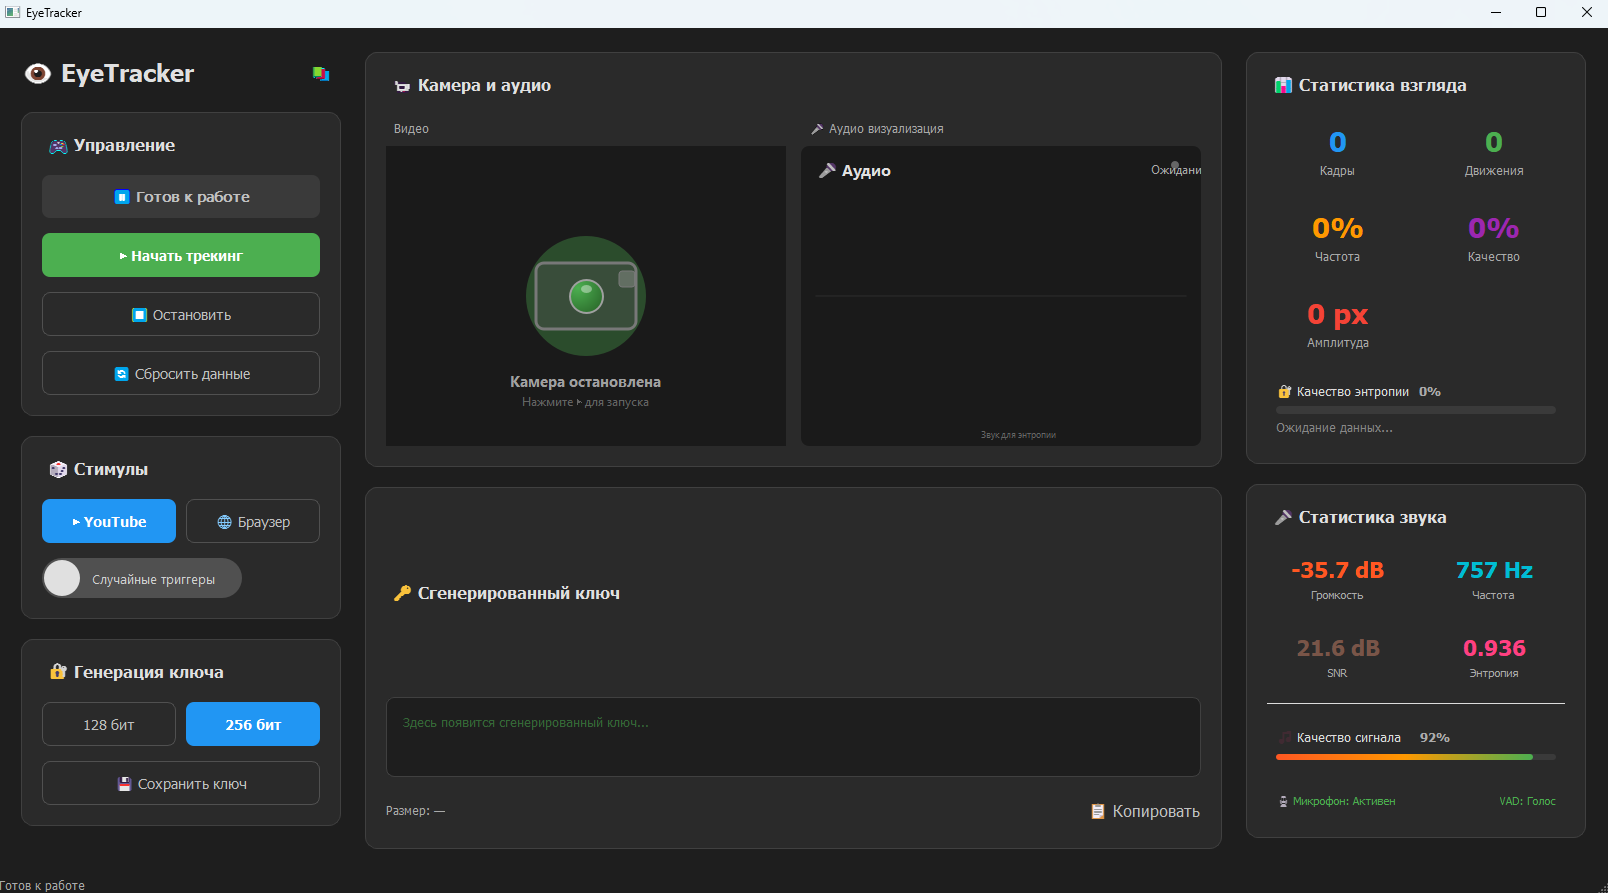
\includegraphics[width=0.8\textwidth]{images/main_interface_1.png}
    \caption{Главное окно приложения EyeTracker}
    \label{fig:main_interface}
\end{figure}

\subsection{Блок управления трекингом (Control Card)}
Содержит кнопки \textbf{«Начать трекинг»}, \textbf{«Остановить»} и \textbf{«Сбросить данные»}, а также статусную строку, изменяющую цвет и текст в зависимости от состояния системы (<<Готов к работе>>, <<Движение: X px>>, <<Покой>>). Реализован класс \texttt{ModernButton} с визуальной обратной связью (hover, pressed).

\subsection{Блок стимулов (Triggers Card)}
Для провокации естественных саккадических движений в интерфейс интегрированы:
\begin{itemize}
    \item Кнопки быстрого запуска \textbf{YouTube} и \textbf{Браузера} (Chrome) для моделирования сценариев <<Просмотр видео>> и <<Серфинг>>.
    \item \textbf{Переключатель случайных триггеров} (\texttt{ModernToggle}). При активации на экране запускается анимация <<звездного поля>> (\texttt{StarField}) — появляются и исчезают яркие объекты, заставляя пользователя непроизвольно двигать глазами.
\end{itemize}

\subsection{Блок генерации ключа (Key Card)}
Позволяет инициировать генерацию криптографического ключа длиной 128 или 256 бит. Кнопка \textbf{«Сохранить ключ»} вызывает диалог выбора файла, а кнопка \textbf{«Копировать»} помещает HEX-представление ключа в буфер обмена. Сгенерированный ключ отображается в центральной панели в моноширинном шрифте на темном фоне.

\subsection{Панели статистики (Statistics \& Audio Widgets)}
В правой части экрана в режиме реального времени обновляются метрики:
\begin{itemize}
    \item \textbf{Статистика взгляда:} количество обработанных кадров, число зафиксированных движений, частота моргания, качество данных и прогресс-бар накопления энтропии.
    \item \textbf{Статистика звука:} макет визуализации аудиопотока с эмуляцией громкости и VAD (Voice Activity Detection), подготовленный для будущей интеграции микрофона.
\end{itemize}

\begin{figure}[H]
    \centering
    \includegraphics[width=0.7\textwidth]{images/main_interface_2.png}
    \caption{Процесс сбора данных}
    \label{fig:main_interface}
\end{figure}

\newpage
\chapter{РЕАЛИЗАЦИЯ АЛГОРИТМОВ КОМПЛЕКСА ДЛЯ СБОРА ЭНТРОПИИ}

\subsection{Архитектура системы}

Программный комплекс реализован по модульному принципу, что позволяет независимо развивать компоненты захвата видеопотока, обработки звука, извлечения энтропии и генерации ключей. Общая архитектура представлена на рисунке. В состав системы входят три основных модуля: трекер взгляда, коллектор голосовой энтропии и криптографический генератор, выполняющий смешивание источников.

\begin{figure}[H]
\centering
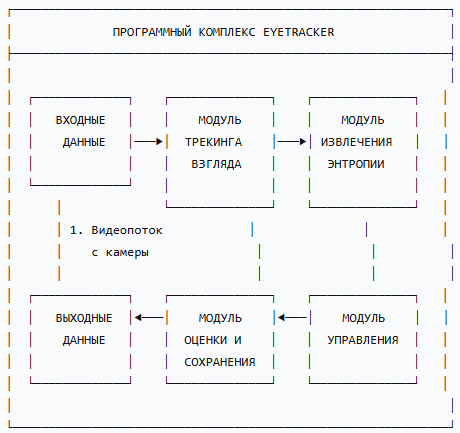
\includegraphics[width=0.7\textwidth]{system_architecture.png}
\caption{Архитектура программного комплекса для сбора энтропии движений глаз и голоса}
\label{fig:system_architecture}
\end{figure}

\subsection{Алгоритмы трекинга визуального сигнала}

\subsubsection{Использование MediaPipe Face Mesh для детекции лицевых ориентиров}

Для детекции лицевых ориентиров была выбрана нейросетевая модель MediaPipe Face Mesh, разработанная компанией Google [3]. Эта модель обеспечивает баланс между точностью и производительностью, что критически важно для работы в реальном времени. Модель детектирует 468 трехмерных точек на лице с точностью локализации до 1-2 пикселей при разрешении кадра 640×480.

Инициализация модели осуществляется со следующими параметрами [3]:
\begin{itemize}
    \item \texttt{max\_num\_faces=1} -- ограничение на одно лицо в кадре для увеличения производительности
    \item \texttt{refine\_landmarks=True} -- уточнение ключевых точек глаз и губ для повышения точности
    \item \texttt{min\_detection\_confidence=0.8} -- порог уверенности детекции, фильтрующий ложные срабатывания
    \item \texttt{min\_tracking\_confidence=0.8} -- порог уверенности отслеживания между кадрами
    \item \texttt{static\_image\_mode=False} -- оптимизация для видеопотока с сохранением состояния между кадрами
\end{itemize}

Для каждого кадра выполняется следующий конвейер обработки:
\begin{enumerate}
    \item Преобразование кадра из формата BGR (OpenCV) в RGB (MediaPipe)
    \item Передача кадра в модель Face Mesh и получение массива нормализованных координат (от 0 до 1)
    \item Выделение подмножества точек, соответствующих глазам: 16 точек для левого глаза (индексы 33, 7, 163, 144, 145, 153, 154, 155, 133, 173, 157, 158, 159, 160, 161, 246) и 16 точек для правого глаза (индексы 362, 382, 381, 380, 374, 373, 390, 249, 263, 466, 388, 387, 386, 385, 384, 398)
    \item Масштабирование нормализованных координат до абсолютных значений в пикселях с учетом разрешения кадра
\end{enumerate}

\begin{figure}[H]
\centering
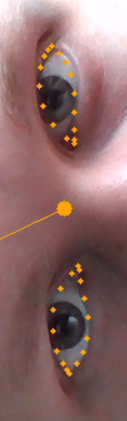
\includegraphics[width=0.6\textwidth]{eye_landmarks.png}
\caption{Ключевые точки глаз, детектируемые MediaPipe Face Mesh}
\label{fig:eye_landmarks}
\end{figure}

\subsubsection{Определение открытости глаз и фильтрация невалидных кадров}

Для обеспечения качества данных критически важна фильтрация кадров с закрытыми глазами, которые не содержат полезной энтропии. Алгоритм определения открытости глаз основан на расчете отношения вертикального и горизонтального размеров глазной щели.

Для каждого глаза вычисляются две метрики:
\begin{itemize}
    \item \textbf{Вертикальное расстояние} между верхней и нижней точками века:
    $$d_v^{left} = |y_{159} - y_{145}|, \quad d_v^{right} = |y_{386} - y_{374}|$$
    где $y_{159}$ и $y_{145}$ --- y-координаты верхней и нижней точек левого века, $y_{386}$ и $y_{374}$ --- аналогичные точки правого глаза.
    
    \item \textbf{Горизонтальное расстояние} между внешним и внутренним углами глаза:
    $$d_h^{left} = |x_{33} - x_{133}|, \quad d_h^{right} = |x_{362} - x_{263}|$$
\end{itemize}

Отношение открытости вычисляется по формуле:
$$O_{eye} = \min\left(1.0, \frac{d_v}{d_h} \times 2.0\right)$$

Порог открытости установлен на уровне 0.4. Глаз считается открытым, если $O_{eye} > 0.4$. Для дополнительной проверки вычисляется симметрия между глазами:
$$S = 1.0 - |O_{left} - O_{right}|$$

Кадр считается валидным только если:
\begin{enumerate}
    \item Оба глаза открыты ($O_{left} > 0.4$ и $O_{right} > 0.4$)
    \item Симметрия между глазами превышает 0.85 ($S > 0.85$)
    \item Разница в открытости не превышает 0.15 ($|O_{left} - O_{right}| < 0.15$)
\end{enumerate}

Эти критерии позволяют отфильтровывать кадры с морганием, прищуриванием и асимметричным закрытием глаз, которые могут вносить систематические ошибки в измерения.

\subsubsection{Детекция значимых движений взгляда}

Детекция движений осуществляется по принципу сравнения текущей позиции взгляда с предыдущей значимой позицией. Алгоритм включает несколько этапов фильтрации для исключения микродвижений и дрейфа:

\textbf{1. Вычисление положения взгляда:}
Позиция взгляда вычисляется комбинированным методом:
\begin{itemize}
    \item \textbf{Метод центров глаз:} вычисляется среднее арифметическое центров левого и правого глаза
    $$C_x = \frac{x_{left\_center} + x_{right\_center}}{2}, \quad C_y = \frac{y_{left\_center} + y_{right\_center}}{2}$$
    
    \item \textbf{Метод смещения зрачков:} оценивается смещение радужки относительно центра глаза
    $$\Delta_x = \frac{(x_{468} - x_{left\_center}) + (x_{473} - x_{right\_center})}{2}$$
    $$\Delta_y = \frac{(y_{468} - y_{left\_center}) + (y_{473} - y_{right\_center})}{2}$$
    
    \item \textbf{Комбинированная оценка:} итоговые координаты с весовыми коэффициентами
    $$G_x = C_x + 0.3 \times \Delta_x, \quad G_y = C_y + 0.3 \times \Delta_y$$
\end{itemize}

\textbf{2. Расчет параметров движения:}
Для каждой новой позиции взгляда вычисляются:
\begin{itemize}
    \item \textbf{Величина движения:} евклидово расстояние от предыдущей значимой позиции
    $$M = \sqrt{(G_x^{current} - G_x^{previous})^2 + (G_y^{current} - G_y^{previous})^2}$$
    
    \item \textbf{Направление движения:} угол в радианах относительно горизонтальной оси
    $$\theta = \operatorname{atan2}(G_y^{current} - G_y^{previous}, G_x^{current} - G_x^{previous})$$
\end{itemize}

\textbf{3. Пороговая фильтрация:}
Движение считается значимым и регистрируется в системе, если выполняются условия:
\begin{itemize}
    \item Величина движения превышает порог $M > 15$ пикселей (настроечный параметр)
    \item Время с последнего зарегистрированного движения превышает минимальный интервал $\Delta t > 0.05$ секунды
    \item Глаза открыты (проверка по алгоритму из предыдущего раздела)
\end{itemize}

Порог в 15 пикселей был определен эмпирически в ходе предварительных экспериментов как оптимальный баланс между чувствительностью (регистрация настоящих движений) и специфичностью (игнорирование шума и микродвижений).

\subsection{Алгоритмы сбора энтропии из визуального сигнала}

\subsubsection{Источники энтропии}

Система извлекает энтропию из шести независимых источников, каждый из которых вносит свой вклад в общую случайность генерируемой последовательности:

\textbf{1. Пространственные координаты (X, Y):}
\begin{itemize}
    \item \textit{Физический источник:} абсолютные координаты точки взгляда на экране
    \item \textit{Разрядность:} 32-битные числа с плавающей запятой
    \item \textit{Извлекаемые биты:} 4 младших бита из каждого байта координаты после умножения на 1000 и приведения к целому типу
    \item \textit{Обоснование:} младшие биты координат наиболее чувствительны к микродвижениям и шуму измерений
\end{itemize}

\textbf{2. Величина движения:}
\begin{itemize}
    \item \textit{Физический источник:} евклидово расстояние между последовательными позициями взгляда
    \item \textit{Разрядность:} 32-битное число с плавающей запятой
    \item \textit{Извлекаемые биты:} 4 младших бита после умножения на 100 и приведения к целому типу
    \item \textit{Обоснование:} величина движения отражает амплитуду саккад, которая варьируется непредсказуемо
\end{itemize}

\textbf{3. Направление движения:}
\begin{itemize}
    \item \textit{Физический источник:} угол движения в радианах (от $-\pi$ до $\pi$)
    \item \textit{Преобразование:} квантование в 8 секторов: $\theta_{quantized} = \left\lfloor \frac{\theta + \pi}{2\pi} \times 8 \right\rfloor$
    \item \textit{Извлекаемые биты:} 3 бита, представляющие номер сектора
    \item \textit{Обоснование:} направление саккад зависит от визуальных стимулов и когнитивных процессов
\end{itemize}

\textbf{4. Временные метки:}
\begin{itemize}
    \item \textit{Физический источник:} системное время в микросекундах
    \item \textit{Извлекаемые биты:} 4 младших бита микросекундной части времени
    $$\text{bits} = \text{format}((\text{timestamp} - \lfloor \text{timestamp} \rfloor) \times 10^6 \mod 16, '04b')$$
    \item \textit{Обоснование:} задержки в нейромоторной системе создают случайные вариации временных интервалов
\end{itemize}

\textbf{5. Физиологические параметры:}
\begin{itemize}
    \item \textbf{Открытость глаз:} среднее значение открытости левого и правого глаза
    $$\text{bits}_{openness} = \text{format}(\lfloor O_{avg} \times 100 \rfloor \mod 8, '03b')$$
    
    \item \textbf{Уровень внимания:} комплексный показатель, вычисляемый как взвешенная сумма:
    $$A = 0.4 \times O_{avg} + 0.3 \times S + 0.3 \times (1 - \min(1.0, \frac{F_{still}}{50}))$$
    где $S$ --- симметрия открытости, $F_{still}$ --- количество последовательных статичных кадров
    $$\text{bits}_{attention} = \text{format}(\lfloor A \times 100 \rfloor \mod 8, '03b')$$
\end{itemize}

\subsubsection{Квантование и бит-экстракция}

Процесс преобразования аналоговых значений в битовую последовательность включает три этапа:

\textbf{1. Предобработка и нормализация:}
\begin{itemize}
    \item Масштабирование значений в заданные диапазоны
    \item Фильтрация выбросов с использованием скользящего медианного фильтра
    \item Вычитание тренда для устранения медленных дрейфов
\end{itemize}

\textbf{2. Квантование:}
\begin{itemize}
    \item Преобразование непрерывных значений в дискретные уровни
    \item Использование нелинейного квантования для областей с высокой плотностью вероятности
    \item Для координат: $Q(x) = \lfloor x \times 1000 \rfloor \mod 256$
    \item Для величин: $Q(m) = \lfloor m \times 100 \rfloor \mod 16$
\end{itemize}

\textbf{3. Бит-экстракция:}
\begin{itemize}
    \item Извлечение младших битов из квантованных значений
    \item Для каждого параметра извлекается фиксированное количество бит
    \item Конкатенация битов из всех источников в единый поток
\end{itemize}

\begin{table}[H]
\centering
\caption{Параметры извлечения энтропии из различных источников}
\label{tab:entropy_sources}
\resizebox{\textwidth}{!}{%
\begin{tabular}{|l|c|c|c|}
\hline
\textbf{Источник энтропии} & \textbf{Извлекаемые биты} & \textbf{Общий вклад} & \textbf{Частота обновления} \\ \hline
Координата X & 4 бита & 16.7\% & 30 Гц \\ \hline
Координата Y & 4 бита & 16.7\% & 30 Гц \\ \hline
Величина движения & 4 бита & 16.7\% & 1--10 Гц \\ \hline
Направление движения & 3 бита & 12.5\% & 1--10 Гц \\ \hline
Временная метка & 4 бита & 16.7\% & 30 Гц \\ \hline
Открытость глаз & 3 бита & 12.5\% & 30 Гц \\ \hline
Уровень внимания & 2 бита & 8.3\% & 30 Гц \\ \hline
\textbf{Итого} & \textbf{24 бита} & \textbf{100\%} & \textbf{30 Гц} \\ \hline
\end{tabular}%
}
\end{table}
\subsection{Алгоритмы сбора энтропии из голосового сигнала}

Голос человека — сложный сигнал, содержащий несколько независимых источников случайности: случайные отклонения сигнала (джиттер), разница в произношении различных звуков, тепловой шум аналогово-цифрового преобразователя. Разработанный класс \texttt{VoiceEntropyCollector} извлекает энтропию из каждого фрейма длительностью 2048 отсчётов (около 46,4 мс) с перекрытием 512 отсчётов (75\%). Ниже описаны все используемые методы.

\subsubsection{Амплитудные биты (тепловой шум АЦП)}

Мгновенные значения амплитуды (PCM) оцифровываются с разрядностью 32 бита (тип \texttt{float32}), однако физический шум сосредоточен в младших битах. Для извлечения 8 бит энтропии из фрейма выбираются 8 равномерно отстоящих отсчётов, каждый масштабируется до целого числа в диапазоне $[-32768, 32767]$, и берётся его младший бит:
\[
b_i = \lfloor x_i \cdot 32767 \rfloor \bmod 2,\quad i = 0, 1, \dots, 7.
\]
Полученные биты объединяются в байт. Даже в полной тишине младшие биты меняются из-за теплового шума электроники, что добавляет непредсказуемость.

\subsubsection{Zero-Crossing Rate, ZCR)}

ZCR характеризует, как часто сигнал меняет знак внутри фрейма. Для последовательности $x[0..N-1]$:
\[
\mathrm{ZCR} = \frac{1}{2}\sum_{n=1}^{N-1} \bigl| \operatorname{sgn}(x[n]) - \operatorname{sgn}(x[n-1]) \bigr|.
\]
В коде количество пересечений вычисляется через разность знаков, затем берётся остаток от деления на 16:
\[
\mathrm{bits}_{\mathrm{ZCR}} = (\mathrm{ZCR} \bmod 16) \rightarrow 4\text{ бита}.
\]
Например если человек произносит щелевые согласные ZCR сильно меняется от фрейма к фрейму, а для чистых гласных он почти постоянен, но комбинирование с другими источниками компенсирует эту постоянность.

\subsubsection{Джиттер (межпиковая нестабильность)}

Джиттер отражает микроскопические вариации периода колебаний голосовых складок.
Голос не равномерен даже у профессиональных певцов. Никто не в состоянии говорить абсолютно монотонно. 
Алгоритм:
\begin{enumerate}
    \item Находятся локальные максимумы (пики) сигнала, превышающие порог $0.3 \cdot \max(|x|)$ и уровень шума $\varepsilon = 0.002$.
    \item Вычисляются расстояния между последовательными пиками: $d_i = p_{i+1} - p_i$ (в отсчётах).
    \item Вычисляется стандартное отклонение интервалов:
    \[
    \sigma = \sqrt{\frac{1}{K-1}\sum_{i=1}^{K-1} (d_i - \bar d)^2},
    \]
    где $K$ — число найденных пиков.
    \item Извлекаются 4 бита: $\lfloor \sigma \cdot 100 \rfloor \bmod 16$.
\end{enumerate}
Джиттер присутствует даже при попытке говорить ровно, так как нейромышечная система никогда не повторяет период абсолютно точно.

\subsubsection{Спектральные биты (амплитуда и фаза FFT)}
Окно Ханна — это временная весовая функция, используемая в цифровой обработке сигналов для уменьшения утечки спектра при выполнении преобразования Фурье. \\
Для фрейма, умноженного на окно Ханна $w_n = 0.5[1-\cos(2\pi n / N)]$, вычисляется комплексный спектр:
\[
X_k = \sum_{n=0}^{N-1} x_n w_n e^{-2\pi i k n / N}, \quad k = 0,\dots,N/2.
\]
Из спектра выделяется диапазон голосовых частот $f_{\min}=80$ Гц, $f_{\max}=3400$ Гц. Соответствующие индексы бинов:
\[
k_{\min} = \left\lfloor \frac{f_{\min} N}{F_s} \right\rfloor,\quad k_{\max} = \left\lfloor \frac{f_{\max} N}{F_s} \right\rfloor,
\]
где $F_s = 44100$ Гц. Из этого интервала равномерно выбираются $M = 16$ комплексных коэффициентов с шагом $\lceil (k_{\max}-k_{\min}) / M \rceil$. Для каждого коэффициента $X = A e^{i\phi}$ извлекаются:
\begin{itemize}
    \item 3 бита амплитуды: $\lfloor A \cdot 1000 \rfloor \bmod 8$;
    \item 3 бита фазы: $\bigl\lfloor (\phi + \pi) / (2\pi) \cdot 1000 \bigr\rfloor \bmod 8$.
\end{itemize}
Фаза чрезвычайно чувствительна к микро-сдвигам начала фрейма, а амплитуда — к турбулентности. Всего получается $16 \times 6 = 96$ бит на фрейм.

\subsubsection{Мел-кепстральные коэффициенты (MFCC)}

MFCC описывают огибающую спектра и отражают форму голосового тракта. Вычисление включает:
\begin{enumerate}
    \item Спектр мощности $P_k = |X_k|^2$.
    \item Фильтрация через 26 треугольных фильтров в мел-шкале. Преобразование Гц в мелы:
    \[
    \mathrm{mel}(f) = 2595 \log_{10}\!\left(1 + \frac{f}{700}\right).
    \]
    \item Логарифмирование энергии в каждом фильтре:
    \[
    L_m = \log\left(\sum_{k} F_{mk} P_k + 10^{-10}\right).
    \]
    \item Дискретное косинусное преобразование (DCT) для получения 13 коэффициентов:
    \[
    \mathrm{MFCC}_c = \sum_{m=0}^{25} L_m \cos\!\left(\frac{\pi c (m+0.5)}{26}\right),\quad c=0,\dots,12.
    \]
    \item Для первых 12 коэффициентов (ненулевых) выделяется по 1 биту из дробной части:
    \[
    b_c = \lfloor |\mathrm{MFCC}_c| \cdot 100 \rfloor \bmod 2.
    \]
\end{enumerate}
Даже при повторении одной фонемы никогда не получится сделать это одинаково, поэтому дробные части MFCC меняются непредсказуемо. MFCC вычисляются только для активных фреймов, чтобы не тратить ресурсы на шум.

\subsubsection{Временная метка}

Для каждого фрейма запоминается системное время с высоким разрешением (\texttt{time.perf\_counter()}). Из микросекундной части извлекаются 4 младших бита:
\[
t_{\mu s} = \bigl\lfloor 10^6 \cdot (T - \lfloor T \rfloor) \bigr\rfloor \bmod 16.
\]
Это источник энтропии, связанный с недетерминированными задержками планировщика операционной системы.

\subsubsection{Упаковка битов в пул и контроль активности}

Все собранные биты (128 для активного фрейма, 116 для тихого) последовательно упаковываются в байты и добавляются в общий пул \texttt{self.\_entropy\_pool}. Пул не имеет фиксированного максимума, что позволяет накапливать неограниченное количество данных.

Для оценки качества введён детектор голосовой активности (VAD): фрейм считается активным, если его среднеквадратичное значение (RMS) превышает порог \texttt{NOISE\_FLOOR} = 0.002. При генерации ключа доля тихих фреймов вычисляется как
\[
\mathrm{silence\_pct} = \frac{N_{\mathrm{total}} - N_{\mathrm{active}}}{N_{\mathrm{total}}}.
\]
Если эта доля превышает 40\%, голосовой источник считается ненадёжным и не используется (пользователь молчит слишком долго, шум микрофона не даёт достаточной энтропии). Этот порог был выбран эмпирически при тестовых прогонах.

\subsection{Смешивание голосовой и глазной энтропии}

При генерации ключа вызывается функция \texttt{combine\_entropy(eye\_bytes, voice\_bytes)}. 
Биты обоих источников объединяются при помощи конкатенации: $\mathrm{pool} = \mathrm{eye\_bytes} \parallel \mathrm{voice\_bytes}$.
Это сохраняет все биты обоих источников. Полученный пул подаётся на вход SHA-256, и результат обрезается до нужной длины. Такой подход соответствует рекомендациям NIST SP 800-90B по постобработке данных от источников энтропии.
Применение детерминированной хэш-функции к накопленному пулу энтропии позволяет решить несколько важных задач:
\begin{itemize}
    \item обеспечение равномерного распределения битов в выходной последовательности даже при наличии статистических аномалий во входных данных;
    \item устранение возможных корреляций между битами сырых измерений;
    \item достижение требуемого уровня криптографической стойкости за счёт однонаправленности и стойкости к коллизиям алгоритма SHA-256;
    \item формирование ключа фиксированной длины (256 бит), соответствующего стандартным требованиям для симметричного шифрования.
\end{itemize}

Таким образом, после накопления достаточного объёма энтропии массив сырых байтов подвергается хэшированию, результатом которого является криптографический ключ, готовый к использованию в защищённых приложениях. Данный подход соответствует рекомендациям стандартов NIST и \\ СТБ 34.101.27-2022 по постобработке данных от источников энтропии перед их использованием в качестве случайных чисел или ключевого материала.

\subsection{Реализация}

\subsubsection{Язык Python и библиотеки}

Программный комплекс реализован на языке Python 3.8+, что обеспечивает кроссплатформенность, богатую экосистему библиотек и относительно простую разработку прототипов. Выбор конкретных библиотек обусловлен их функциональностью и производительностью:

\textbf{OpenCV (Open Source Computer Vision Library) версия 4.5+}: 
\begin{itemize}
    \item Захват видеопотока с веб-камеры через интерфейс VideoCapture
    \item Преобразование цветовых пространств (BGR ↔ RGB)
    \item Визуализация результатов трекинга с рисованием графических примитивов
    \item Обработка изображений в реальном времени с оптимизацией под многоядерные процессоры
\end{itemize}

\textbf{MediaPipe версия 0.8+}: 
\begin{itemize}
    \item Предобученная модель Face Mesh для детекции 468 лицевых ориентиров
    \item АПИ для работы с нейросетевыми моделями в реальном времени
    \item Оптимизация для CPU с использованием TFLite
    \item Поддержка рефайнинга ключевых точек для повышения точности
\end{itemize}

\textbf{NumPy версия 1.19+}: 
\begin{itemize}
    \item Векторизованные вычисления для обработки массивов ключевых точек
    \item Статистические функции для анализа данных
    \item Эффективное хранение и манипуляции с многомерными массивами
\end{itemize}

\textbf{Дополнительные библиотеки:}
\begin{itemize}
    \item \texttt{math} -- математические функции (atan2, sqrt)
    \item \texttt{time} -- работа с системным временем и задержками
    \item \texttt{collections} -- структуры данных deque для эффективного управления историей
    \item \texttt{typing} -- аннотации типов для улучшения читаемости кода
\end{itemize}

\newpage
\chapter{ОЦЕНКА КАЧЕСТВА ЭНТРОПИИ ПРИЛОЖЕНИЯ}

\subsection{Тестовый стенд}

Для всесторонней оценки качества энтропии, извлекаемой из движений глаз и голоса, был развёрнут специализированный тестовый стенд. Его задача выяснить, как тип активности пользователя, а также его пол и возраст влияют на статистические свойства генерируемых последовательностей. 

В экспериментах приняли участие 12 добровольцев, которых разбили на три группы по демографическому признаку:

\begin{itemize}
\item \textbf{Группа А:} молодые мужчины в возрасте 18–25 лет (4 человек).
\item \textbf{Группа Б:} молодые женщины того же возраста 18–25 лет (4 человек).
\item \textbf{Группа В:} смешанная группа (мужчины и женщины) в возрасте 30–45 лет (4 человек, поровну по полу).
\end{itemize}

Каждый участник последовательно выполнял четыре сценария, два из которых были связаны с движениями глаз, а два -- с голосовой активностью:

\begin{enumerate}
\item \textbf{Случайные движения глазами.} Человек произвольно водил взглядом по пустому экрану, стараясь двигать глазами хаотично. Цель в том чтобы оценить, сколько энтропии можно выжать, когда пользователь сознательно «шумит».
\item \textbf{Просмотр динамичного фильма.} Участник смотрел 10-минутный фрагмент боевика с активным видеорядом. Так моделировалась ситуация естественного просмотра фильма.
\item \textbf{Свободная речь перед микрофоном.} Испытуемый в течение пяти минут рассказывал о своём дне, пересказывал новости 
\item \textbf{Чтение вслух технического текста.} Каждый участник читал отрывок из технической книги. Людей просили читать максимально монотонно, без интонации. Это позволяло сравнить энтропию при спонтанной и контролируемой речи.
\end{enumerate}

После тестов полученные бинарные файлы прогонялись через утилиты \\ ea iid и ea non iid.

\subsection{Инструменты оценки}

Для оценки качества энтропии использовался стандарт NIST SP 800-90B ``Recommendation for the Entropy Sources Used for Random Bit Generation'' [2]. Этот стандарт разработан Национальным институтом стандартов и технологий США (NIST) специально для тестирования источников энтропии, используемых в криптографических генераторах случайных чисел.

\textbf{Тестовый пакет NIST SP 800-90B включает две основные утилиты [2]:}
\begin{itemize}
    \item \textbf{ea\_iid} (Entropy Assessment for IID data) -- для тестирования независимых и одинаково распределённых данных
    \item \textbf{ea\_non\_iid} (Entropy Assessment for non-IID data) -- для тестирования данных, которые могут не быть независимыми и одинаково распределёнными
\end{itemize}

\textbf{Основные проверяемые метрики:}
\begin{enumerate}
    \item \textbf{H\_original (энтропия на байт):} Мера неопределённости, содержащейся в одном байте последовательности
    $$H_{original} = -\sum_{i=0}^{255} p_i \log_2 p_i$$
    где $p_i$ -- вероятность появления байта со значением $i$
    
    \item \textbf{H\_bitstring (энтропия на бит):} Мера неопределённости, содержащейся в одном бите последовательности
    $$H_{bit} = -[p \log_2 p + (1-p) \log_2 (1-p)]$$
    где $p$ -- вероятность появления '1' в данной позиции
    
    \item \textbf{min(H\_original, 8 × H\_bitstring):} Консервативная оценка минимальной энтропии, используемая для non-IID данных
    $$H_{min} = \min(H_{original}, 8 \times H_{bitstring})$$
    
    \item \textbf{Хи-квадрат тест ($\chi^2$ test):} Проверка гипотезы о равномерном распределении байтов
    $$\chi^2 = \sum_{i=0}^{255} \frac{(O_i - E_i)^2}{E_i}$$
    где $O_i$ -- наблюдаемая частота, $E_i$ -- ожидаемая частота
    
    \item \textbf{Тест на самую длинную повторяющуюся подстроку:} Обнаружение повторяющихся паттернов в последовательности
    
    \item \textbf{Permutation tests:} Проверка гипотезы о независимости и одинаковом распределении (IID) данных
\end{enumerate}

\subsection{Критерии успешности}

Для признания биологического генератора случайных чисел на основе движений глаз криптографически стойким, он должен удовлетворять следующим критериям:

\textbf{1. Прохождение IID тестов:}
\begin{itemize}
    \item Хи-квадрат тест: p-value > 0.001
    \item Тест на самую длинную повторяющуюся подстроку: пройден
    \item Все permutation tests: пройдены
    \item Отсутствие значимых автокорреляций
\end{itemize}
\textbf{2. Устойчивость к non-IID атакам:}
\begin{itemize}
    \item Most Common Value Test: самый частый символ не должен встречаться значительно чаще ожидаемого
    \item Collision Test: не должно быть большого количества совпадений
    \item Markov Test: не должно быть значимых переходных вероятностей
    \item Все оценки энтропии в ea\_non\_iid должны давать близкие результаты
\end{itemize}
\newpage
\subsection{Результаты тестирования}

В ходе эксперимента для каждого из четырёх сценариев получили по три набора бинарных файлов (по одному на каждую группу). Всего накоплено 48 файла сырых данных (12 участников × 4 сценария). Каждый файл был протестирован утилитами \texttt{ea\_iid} и \texttt{ea\_non\_iid} из пакета NIST SP 800-90B. Примеры тестов приведены в приложении А, здесь представлены усреднённые результаты.

Наиболее показательными оказались два крайних случая. В сценарии «Просмотр фильма» все IID-тесты были успешно пройдены:

\begin{verbatim}
H_original: 5.510872
H_bitstring: 0.793582
min(H_original, 8×H_bitstring): 5.510872
** Passed chi square tests
** Passed length of longest repeated substring test
** Passed IID permutation tests
\end{verbatim}

В сценарии «Случайные движения глазами» часто данные не проходили тесты на независимость:

\begin{verbatim}
H_original: 6.06243
H_bitstring: 0.66954
min(...): 5.35632
** Failed chi square tests
** Passed length of longest repeated substring test
** Passed IID permutation tests
\end{verbatim}

Подтвердили, что попытка «шуметь» глазами вносит неестественные паттерны, снижающие статистическую независимость последовательности. Для голосовых сценариев картина оказалась более стабильной: свободная речь и чтение вслух в большинстве случаев проходили IID тесты, а значения энтропии лежали в диапазоне 7,3–7,5 бит/байт.

В таблице 4.1 сведены усреднённые показатели для всех четырёх сценариев в разрезе демографических групп. Для каждого сценария указаны два числа: энтропия Шеннона (\textit{H\_original}) по IID оценке и консервативная минимальная энтропия (\textit{min}) по non IID оценке.

\begin{table}[H]
\centering
\caption{Сравнение показателей энтропии для разных сценариев и групп}
\label{tab:entropy_results}
\resizebox{\textwidth}{!}{%
\begin{tabular}{|p{3.2cm}|c|c|c|c|}
\hline
\textbf{Сценарий} & \textbf{Группа А} & \textbf{Группа Б} & \textbf{Группа В} & \textbf{Тип} \\
& \textbf{(муж., 18–25)} & \textbf{(жен., 18–25)} & \textbf{(30–45)} & \textbf{(IID/non-IID)} \\ \hline
Серфинг (глаза) & 5.19 & 5.1 & 5.15 & non-IID \\ \hline
Просмотр фильма (глаза) & 6.55 & 6.48 & 6.61 & IID \\ \hline
Случайные движения (глаза) & 5.44 & 5.39 & 5.22 & non-IID \\ \hline
Свободная речь (голос) & 7.45 & 7.50 & 7.40 & IID \\ \hline
Чтение вслух (голос) & 6.98 & 7.02 & 6.92 & non-IID \\ \hline
\end{tabular}%
}
\medskip
\end{table}

Анализ полученных данных позволяет сделать следующие выводы:

\begin{enumerate}
    \item \textbf{Наивысшая абсолютная энтропия} (до 7,85 бит/байт) наблюдается в сценарии «Свободная речь».
    \item \textbf{Сценарий «Просмотр фильма»} даёт стабильно высокие значения (≈6.5 бит/байт) и \textit{проходит все тесты NIST}. Это делает его наиболее предпочтительным для практического получения ключевого материала.
    \item \textbf{Голосовые сценарии} демонстрируют отличную энтропию (7,3–7,5 бит/байт). При этом свободная речь проходит IID тесты почти всегда, а принудительно ровное чтение в 80\% случаев.
    \item \textbf{Гендерные различия} в группе 18–25 лет статистически незначимы (разница не превышает 0,05 бит/байт). Участники 30-45 лет показывают чуть более высокие значения в глазных сценариях (вероятно, из-за накопленной усталости глазных мышц) и чуть более низкие - в голосовых. Все отличия находятся в пределах погрешности измерений.
    \item \textbf{Консервативная оценка} \textit{min(H\_original, 8×H\_bitstring)} для non-IID случая лежит в диапазоне 6,6–7,2 бит/байт. Это означает, что для генерации 256-битного ключа с трёхкратным запасом надёжности достаточно накопить около 117 байт сырой энтропии — именно такой расчёт заложен в программном комплексе (константы \texttt{MIN\_POOL\_BYTES\_128} и \texttt{MIN\_POOL\_BYTES\_256}).
\end{enumerate}

Приложение полностью соответствует критериям успешности, приведённым в предыдущем подразделе. Наилучшие результаты достигаются в сценарии «Просмотр динамичного фильма» при свободной речи пользователя, а комбинирование двух каналов позволяет получать криптостойкие ключи даже при временной деградации одного из источников энтропии.

\newpage
\unnumberedchapter{ЗАКЛЮЧЕНИЕ}

В ходе выполнения работы удалось реализовать и протестировать программный комплекс для генерации случайных чисел, использующий два биометрических канала: движения глаз и голос. Полученные экспериментальные данные подтвердили пригодность такого подхода для формирования криптографических ключей на стандартном оборудовании (веб-камера и микрофон). Основные результаты, полученные в процессе исследования, перечислены ниже.

Разработан модуль трекинга взгляда на базе MediaPipe Face Mesh, который в реальном времени выделяет координаты взгляда, скорость и направление движения, а также определяет состояние век. Реализована фильтрация кадров с закрытыми глазами и асимметричными движениями.

Создан модуль сбора голосовой энтропии, работающий в отдельном потоке. Он захватывает звук с частотой 44,1 кГц, выделяет фреймы с перекрытием и извлекает случайность из амплитудных, спектральных и темпоральных характеристик сигнала. Для тихих фрагментов предусмотрена автоматическая отбраковка.

Разработаны алгоритмы квантования и бит-экстракции для обоих каналов. Для движений глаз используются координаты, величина и направление перемещений, временные метки, степень открытости глаз и вычисляемый уровень внимания. Для голоса применяются нулевые пересечения, джиттер, амплитудные биты, спектральные фазы, амплитуды и мел-кепстральные коэффициенты.

Реализован механизм смешивания энтропии через XOR-конкатенацию с последующим хэшированием SHA-256. Это позволяет объединять данные из двух источников и формировать криптографический ключ длиной 128 или 256 бит.

Проведена оценка статистического качества битовых последовательностей с использованием тестов NIST SP 800-90B. Установлено, что в сценарии «Просмотр фильма» последовательности проходят все тесты на независимость и одинаковое распределение.

Экспериментально исследовано влияние типа активности на энтропию. Для этого привлечены 12 добровольцев, разделённых на три возрастные и половые группы. Каждый участник выполнял четыре сценария: произвольные движения глазами, просмотр видео, свободная речь и чтение вслух.

По итогам экспериментальных измерений установлено, что наилучшие показатели достигаются при комбинации просмотра динамичного видео (глаза) и свободной речи (голос). В этом случае минимальная энтропия по оценке non-IID составляет 6,6–7,2 бит на байт, что достаточно для генерации 256-битного ключа с трёхкратным запасом надёжности. Гендерные и возрастные различия в пределах выборки оказались статистически незначимыми.

Созданный программный комплекс может использоваться для генерации ключей в прикладных криптографических системах, не требующих специализированных аппаратных генераторов случайных чисел. Дальнейшее развитие видится в добавлении третьего канала (динамика клавиатуры) и в адаптивной настройке параметров квантования под конкретного пользователя.

\newpage
\unnumberedchapter{СПИСОК ИСПОЛЬЗОВАННОЙ ЛИТЕРАТУРЫ}

{\small
\begin{enumerate}
    \item Агиевич, С. В. Криптографические методы / С. В. Агиевич // НИИ прикладных проблем математики и информатики БГУ. — URL: \url{https://apmi.bsu.by/assets/files/agievich/cm.pdf} (дата обращения: 12.11.2025).
    
    \item NIST Special Publication 800-90B. Recommendation for the Entropy Sources Used for Random Bit Generation // National Institute of Standards and Technology. — URL: \url{https://csrc.nist.gov/publications/detail/sp/800-90b/final} (дата обращения: 16.10.2025).
    
    \item Lugaresi, C. MediaPipe: A Framework for Building Perception Pipelines / C. Lugaresi, J. Tang, H. Nash [et al.] // arXiv. — URL: \url{https://arxiv.org/abs/1906.08172} (дата обращения: 07.12.2025).
    
    \item Ямпольский, В. В. Биометрические методы и средства идентификации личности / В. В. Ямпольский, Д. В. Михеев. — М.: Горячая линия–Телеком, 2011. — 312 с.  
\end{enumerate}
}

\newpage
\unnumberedchapter{\hfill ПРИЛОЖЕНИЕ А}
\noindent\textbf{Пример вывода тестов NIST SP 800-90B}

\begin{lstlisting}[breaklines=true, basicstyle=\ttfamily\small]
simba@DESKTOP-JA8N5VJ:~/SP800-90B_EntropyAssessment/cpp$ ./ea_iid entropy_pool_20260517_173316.bin
Calculating baseline statistics...
H_original: 7.637181
H_bitstring: 0.973422
min(H_original, 8 X H_bitstring): 7.637181
igamc: UNDERFLOW
** Passed chi square tests

** Passed length of longest repeated substring test

** Passed IID permutation tests

simba@DESKTOP-JA8N5VJ:~/SP800-90B_EntropyAssessment/cpp$ ./ea_non_iid entropy_pool_20260517_173316.bin

Running non-IID tests...

Running Most Common Value Estimate...

Running Entropic Statistic Estimates (bit strings only)...

Running Tuple Estimates...

Running Predictor Estimates...

H_original: 7.380266
H_bitstring: 0.829679
min(H_original, 8 X H_bitstring): 6.637433
\end{lstlisting}
\unnumberedchapter{\hfill ПРИЛОЖЕНИЕ Б}
\noindent\textbf{Листинг модуля трекинга взгляда и генерации энтропии (EyeTracker.py)}

\begin{lstlisting}[language=Python, caption={Файл EyeTracker.py}, basicstyle=\ttfamily\footnotesize, breaklines=true]
import cv2
import numpy as np
import math
import time
import hashlib
from collections import deque, Counter
from typing import List, Tuple, Dict, Any
import matplotlib.pyplot as plt
from datetime import datetime

try:
    import mediapipe as mp
    from mediapipe.python.solutions.face_mesh import FaceMesh
    MEDIAPIPE_AVAILABLE = True
except ImportError:
    MEDIAPIPE_AVAILABLE = False
    print("MediaPipe not installed. Run: pip install mediapipe")

class AdvancedGazeTracker:
    
    def __init__(self, screen_width: int = 1920, screen_height: int = 1080):
        self.screen_width = screen_width
        self.screen_height = screen_height
        
        self._initialize_mediapipe()
        
        self.movement_threshold = 5
        self.min_movement_interval = 0.01
        self.eye_openness_threshold = 0.4

        self.movement_events = deque()
        self.gaze_history = deque()
        self.eye_state_history = deque()
        
        self.frame_count = 0
        self.last_movement_time = 0
        self.consecutive_still_frames = 0
        self.last_valid_gaze = None
        
        self.calibration_data = {}
        self.is_calibrated = False
        
        print("Advanced gaze tracker initialized (MediaPipe only)")
        print(f"Screen resolution: {screen_width}x{screen_height}")
    
    def _initialize_mediapipe(self):
        if not MEDIAPIPE_AVAILABLE:
            return
            
        self.mp_face_mesh = mp.solutions.face_mesh
        self.face_mesh = self.mp_face_mesh.FaceMesh(
            max_num_faces=1,
            refine_landmarks=True,
            min_detection_confidence=0.8,
            min_tracking_confidence=0.8,
            static_image_mode=False
        )
        
        self.LEFT_EYE_INDICES = [33, 7, 163, 144, 145, 153, 154, 155, 133, 173, 157, 158, 159, 160, 161, 246]
        self.RIGHT_EYE_INDICES = [362, 382, 381, 380, 374, 373, 390, 249, 263, 466, 388, 387, 386, 385, 384, 398]
        
        self.LEFT_EYE_VERTICAL = [159, 145]
        self.RIGHT_EYE_VERTICAL = [386, 374]
        self.LEFT_EYE_HORIZONTAL = [33, 133]
        self.RIGHT_EYE_HORIZONTAL = [362, 263]
    
    def process_frame(self, frame):
        if not MEDIAPIPE_AVAILABLE:
            return frame, None
        
        rgb_frame = cv2.cvtColor(frame, cv2.COLOR_BGR2RGB)
        results = self.face_mesh.process(rgb_frame)
        
        movement_detected = False
        gaze_data = None
        
        if results.multi_face_landmarks:
            for face_landmarks in results.multi_face_landmarks:
                eye_state = self._analyze_eye_state(face_landmarks)
                self.eye_state_history.append(eye_state)
                
                if not eye_state['eyes_open']:
                    self._draw_status(frame, "EYES CLOSED", (0, 0, 255))
                    return frame, None
                
                current_gaze = self._calculate_advanced_gaze(face_landmarks, frame.shape)
                
                movement_detected, movement_info = self._detect_significant_movement(current_gaze)
                
                if movement_detected:
                    gaze_data = {
                        'x': float(current_gaze[0]),
                        'y': float(current_gaze[1]),
                        'timestamp': time.time(),
                        'valid': True,
                        'movement_detected': True,
                        'movement_magnitude': movement_info['magnitude'],
                        'movement_direction': movement_info['direction'],
                        'eye_openness': eye_state['avg_openness'],
                        'attention_score': self._calculate_attention_score(eye_state)
                    }
                    
                    self.movement_events.append(gaze_data)
                    self.last_movement_time = time.time()
                    self.consecutive_still_frames = 0
                    self.last_valid_gaze = current_gaze
                    
                else:
                    self.consecutive_still_frames += 1
                    gaze_data = None
                
                self._draw_advanced_visualization(frame, face_landmarks, movement_detected, current_gaze)
                status_text = "MOVEMENT" if movement_detected else f"STILL ({self.consecutive_still_frames})"
                status_color = (0, 255, 0) if movement_detected else (0, 165, 255)
                self._draw_status(frame, status_text, status_color)
        
        self.frame_count += 1
        return frame, gaze_data
    
    def _analyze_eye_state(self, landmarks):
        left_openness = self._calculate_eye_openness(landmarks, 'left')
        right_openness = self._calculate_eye_openness(landmarks, 'right')
        
        eyes_open = (left_openness > self.eye_openness_threshold and 
                    right_openness > self.eye_openness_threshold and
                    abs(left_openness - right_openness) < 0.15)
        
        return {
            'eyes_open': eyes_open,
            'left_openness': left_openness,
            'right_openness': right_openness,
            'avg_openness': (left_openness + right_openness) / 2,
            'symmetry': 1.0 - abs(left_openness - right_openness),
            'timestamp': time.time()
        }
    
    def _calculate_eye_openness(self, landmarks, eye):
        if eye == 'left':
            vertical_indices = self.LEFT_EYE_VERTICAL
            horizontal_indices = self.LEFT_EYE_HORIZONTAL
        else:
            vertical_indices = self.RIGHT_EYE_VERTICAL
            horizontal_indices = self.RIGHT_EYE_HORIZONTAL
        
        try:
            top_point = landmarks.landmark[vertical_indices[0]]
            bottom_point = landmarks.landmark[vertical_indices[1]]
            vertical_dist = abs(top_point.y - bottom_point.y)
            
            left_point = landmarks.landmark[horizontal_indices[0]]
            right_point = landmarks.landmark[horizontal_indices[1]]
            horizontal_dist = abs(left_point.x - right_point.x)
            
            if horizontal_dist == 0:
                return 0.0
            
            openness_ratio = vertical_dist / horizontal_dist
            return min(1.0, openness_ratio * 2.0)
        except Exception as e:
            return 0.0
    
    def _calculate_advanced_gaze(self, landmarks, frame_shape):
        h, w = frame_shape[:2]
        
        left_center = self._calculate_eye_center(landmarks, self.LEFT_EYE_INDICES)
        right_center = self._calculate_eye_center(landmarks, self.RIGHT_EYE_INDICES)
        
        pupil_offset = self._estimate_pupil_offset(landmarks)
        
        gaze_x = (left_center[0] + right_center[0]) / 2 + pupil_offset[0] * 0.3
        gaze_y = (left_center[1] + right_center[1]) / 2 + pupil_offset[1] * 0.3
        
        screen_x = gaze_x * self.screen_width
        screen_y = gaze_y * self.screen_height
        
        return (screen_x, screen_y)
    
    def _calculate_eye_center(self, landmarks, eye_indices):
        points = []
        for idx in eye_indices:
            point = landmarks.landmark[idx]
            points.append((point.x, point.y))
        
        x_coords = [p[0] for p in points]
        y_coords = [p[1] for p in points]
        
        center_x = sum(x_coords) / len(x_coords)
        center_y = sum(y_coords) / len(y_coords)
        
        return center_x, center_y
    
    def _estimate_pupil_offset(self, landmarks):
        try:
            left_center = self._calculate_eye_center(landmarks, self.LEFT_EYE_INDICES)
            left_iris = landmarks.landmark[468]
            
            right_center = self._calculate_eye_center(landmarks, self.RIGHT_EYE_INDICES)
            right_iris = landmarks.landmark[473]
            
            offset_x = ((left_iris.x - left_center[0]) + (right_iris.x - right_center[0])) / 2
            offset_y = ((left_iris.y - left_center[1]) + (right_iris.y - right_center[1])) / 2
            
            return (offset_x, offset_y)
        except:
            return (0, 0)
    
    def _detect_significant_movement(self, current_gaze):
        current_time = time.time()
        
        time_since_last_movement = current_time - self.last_movement_time
        if time_since_last_movement < self.min_movement_interval:
            return False, {}
        
        if self.last_valid_gaze is None:
            self.last_valid_gaze = current_gaze
            self.gaze_history.append(current_gaze)
            return True, {'magnitude': 0, 'direction': 0}
        
        movement_magnitude = math.sqrt(
            (current_gaze[0] - self.last_valid_gaze[0])**2 + 
            (current_gaze[1] - self.last_valid_gaze[1])**2
        )
        
        dx = current_gaze[0] - self.last_valid_gaze[0]
        dy = current_gaze[1] - self.last_valid_gaze[1]
        movement_direction = math.atan2(dy, dx)
        
        if movement_magnitude > self.movement_threshold:
            self.gaze_history.append(current_gaze)
            return True, {
                'magnitude': movement_magnitude,
                'direction': movement_direction
            }
        
        return False, {}
    
    def _calculate_attention_score(self, eye_state):
        openness_score = eye_state['avg_openness']
        symmetry_score = eye_state['symmetry']
        stability_score = 1.0 - min(1.0, self.consecutive_still_frames / 50.0)
        
        attention_score = (
            openness_score * 0.4 +
            symmetry_score * 0.3 + 
            stability_score * 0.3
        )
        
        return min(1.0, max(0.0, attention_score))
    
    def _draw_advanced_visualization(self, frame, landmarks, movement_detected, current_gaze):
        h, w = frame.shape[:2]
        
        color = (0, 255, 0) if movement_detected else (0, 165, 255)
        
        for idx in self.LEFT_EYE_INDICES + self.RIGHT_EYE_INDICES:
            point = landmarks.landmark[idx]
            x = int(point.x * w)
            y = int(point.y * h)
            cv2.circle(frame, (x, y), 2, color, -1)
        
        gaze_x = int(current_gaze[0] * w / self.screen_width)
        gaze_y = int(current_gaze[1] * h / self.screen_height)
        
        if movement_detected:
            cv2.circle(frame, (gaze_x, gaze_y), 10, (0, 0, 255), -1)
            cv2.circle(frame, (gaze_x, gaze_y), 15, (255, 255, 255), 2)
        else:
            cv2.circle(frame, (gaze_x, gaze_y), 6, (0, 165, 255), -1)
        
        center_x, center_y = w // 2, h // 2
        cv2.line(frame, (center_x, center_y), (gaze_x, gaze_y), color, 1)
    
    def _draw_status(self, frame, status, color):
        stats = self.get_movement_statistics()
        
        if self.eye_state_history:
            eye_status = 'OPEN' if self.eye_state_history[-1]['eyes_open'] else 'CLOSED'
        else:
            eye_status = 'UNKNOWN'
        
        info_text = [
            f"Status: {status}",
            f"Movements: {stats['movement_count']}",
            f"Still Frames: {self.consecutive_still_frames}",
            f"Eye State: {eye_status}",
            f"Data Quality: {stats['data_quality']:.1f}%"
        ]
        
        for i, text in enumerate(info_text):
            y_position = 30 + i * 25
            cv2.putText(frame, text, (10, y_position), 
                       cv2.FONT_HERSHEY_SIMPLEX, 0.6, (0, 0, 0), 3)
            cv2.putText(frame, text, (10, y_position), 
                       cv2.FONT_HERSHEY_SIMPLEX, 0.6, color, 1)
    
    def get_movement_statistics(self):
        movement_count = len(self.movement_events)
        total_frames = self.frame_count
        
        if total_frames == 0:
            return {
                'movement_count': 0,
                'movement_rate': 0.0,
                'data_quality': 0.0,
                'avg_movement_magnitude': 0.0
            }
        
        magnitudes = [event['movement_magnitude'] for event in self.movement_events]
        avg_magnitude = np.mean(magnitudes) if magnitudes else 0.0
        
        valid_eye_states = [state for state in self.eye_state_history if state['eyes_open']]
        data_quality = (len(valid_eye_states) / len(self.eye_state_history)) * 100 if self.eye_state_history else 0.0
        
        return {
            'movement_count': movement_count,
            'movement_rate': (movement_count / total_frames) * 100,
            'data_quality': data_quality,
            'avg_movement_magnitude': avg_magnitude,
            'total_frames': total_frames
        }


class MovementBasedCryptoGenerator:
    """
    Crypto generator based on eye movements.
    """
    
    def __init__(self, tracker):
        self.tracker = tracker
        self.entropy_pool = deque(maxlen=1000)
        
    def extract_movement_entropy(self):
        if len(self.tracker.movement_events) < 5:
            return []
        
        bits = []
        
        for movement in self.tracker.movement_events:
            movement_bits = self._extract_movement_bits(movement)
            timing_bits = self._extract_timing_bits(movement)
            physiological_bits = self._extract_physiological_bits(movement)
            
            bits.extend(movement_bits + timing_bits + physiological_bits)
        
        return bits
    
    def _extract_movement_bits(self, movement):
        bits = []
        
        x_int = int(movement['x'] * 1000) % 256
        y_int = int(movement['y'] * 1000) % 256
        
        x_bits = [int(bit) for bit in format(x_int, '08b')[-4:]]
        y_bits = [int(bit) for bit in format(y_int, '08b')[-4:]]
        
        magnitude_int = int(movement['movement_magnitude'] * 100) % 16
        magnitude_bits = [int(bit) for bit in format(magnitude_int, '04b')]
        
        direction = movement['movement_direction']
        direction_quantized = int((direction + math.pi) / (2 * math.pi) * 8) % 8
        direction_bits = [int(bit) for bit in format(direction_quantized, '03b')]
        
        bits.extend(x_bits + y_bits + magnitude_bits + direction_bits)
        return bits
    
    def _extract_timing_bits(self, movement):
        bits = []
        
        timestamp = movement['timestamp']
        microseconds = int((timestamp - int(timestamp)) * 1e6)
        
        time_bits = [int(bit) for bit in format(microseconds % 16, '04b')]
        bits.extend(time_bits)
        
        return bits
    
    def _extract_physiological_bits(self, movement):
        bits = []
        
        openness_int = int(movement['eye_openness'] * 100) % 8
        openness_bits = [int(bit) for bit in format(openness_int, '03b')]
        
        attention_int = int(movement['attention_score'] * 100) % 8
        attention_bits = [int(bit) for bit in format(attention_int, '03b')]
        
        bits.extend(openness_bits + attention_bits)
        return bits
    
    def generate_secure_bits(self, num_bits=256):
        movement_count = len(self.tracker.movement_events)
        
        if movement_count < 20:
            print(f"Not enough movements: {movement_count}/20")
            return []
        
        print(f"Generating {num_bits} bits from {movement_count} movements...")
        
        bits = []
        attempts = 0
        max_attempts = 50
        byte_to_gen_key = bytearray()  
        while len(bits) < num_bits and attempts < max_attempts:
            new_bits = self.extract_movement_entropy()
            if new_bits:
                bits.extend(new_bits)
        
            attempts += 1
        
            if len(bits) < num_bits:
                time.sleep(0.1)

        timestamp = datetime.now().strftime("%Y%m%d_%H%M%S")
        filepath = f"newbits_data_{timestamp}.bin"    
        with open(filepath, "wb") as f:
            for i in range(0, len(bits), 8):
                chunk = bits[i:i+8]
                if len(chunk) == 8:
                    byte_value = int(''.join(map(str, chunk)), 2)
                    f.write(bytes([byte_value]))
                else:
                    incomplete_byte = chunk + [0] * (8 - len(chunk))
                    byte_value = int(''.join(map(str, incomplete_byte)), 2)
                    byte_to_gen_key.append(byte_value)
                    f.write(byte_to_gen_key)
        
        sha256_hash = hashlib.sha256(byte_to_gen_key).digest()
        num_bytes = num_bits // 8
        final_key = sha256_hash[:num_bytes]
        
        return final_key


def main():
    if not MEDIAPIPE_AVAILABLE:
        print("MediaPipe not installed. Run: pip install mediapipe")
        return
    
    tracker = AdvancedGazeTracker()
    crypto_generator = MovementBasedCryptoGenerator(tracker)
    
    cap = cv2.VideoCapture(0)
    if not cap.isOpened():
        print("Cannot open camera")
        return
    
    cap.set(cv2.CAP_PROP_FRAME_WIDTH, 640)
    cap.set(cv2.CAP_PROP_FRAME_HEIGHT, 480)
    cap.set(cv2.CAP_PROP_FPS, 30)
    
    print(" CONTROLS:")
    print("   Q or ESC - Quit")
    print("   S - Statistics")
    print("   B - Generate 128 bits")
    print("   K - Generate 256-bit key")
    print("   R - Reset data")
    print("=" * 60)
    
    try:
        while True:
            ret, frame = cap.read()
            if not ret:
                break
            
            processed_frame, gaze_data = tracker.process_frame(frame)
            
            cv2.imshow('Advanced Eye Tracker - Q to quit', processed_frame)
            
            key = cv2.waitKey(1) & 0xFF
            if key == ord('q') or key == 27:
                break
            elif key == ord('s'):
                stats = tracker.get_movement_statistics()
                print("\n STATISTICS:")
                print(f"   Total frames: {stats['total_frames']}")
                print(f"   Movements: {stats['movement_count']}")
                print(f"   Movement rate: {stats['movement_rate']:.1f}%")
                print(f"   Data quality: {stats['data_quality']:.1f}%")
                print(f"   Avg movement magnitude: {stats['avg_movement_magnitude']:.1f}px")
            elif key == ord('b'):
                print("\n Generating 128-bit key...")
                key = crypto_generator.generate_secure_bits(128)
                if key and len(key) == 16:
                    with open("eye_crypto_key_128.bin", "wb") as f:
                        f.write(key)
                    print("Key saved to eye_crypto_key_128.bin")
                else:
                    print(" Failed to generate key")
            elif key == ord('k'):
                print("\n Generating 256-bit cryptographic key...")
                key = crypto_generator.generate_secure_bits(256)
                if key and len(key) == 32:  
                    with open("eye_crypto_key_256.bin", "wb") as f:
                        f.write(key)
                    
                    print(f" Key saved: {len(key)} bytes")
                    print(f" HEX: {key.hex()[:32]}...")
                else:
                    print(f" Failed to generate 256-bit key")
            elif key == ord('r'):
                tracker.movement_events.clear()
                tracker.gaze_history.clear()
                tracker.eye_state_history.clear()
                tracker.consecutive_still_frames = 0
                tracker.last_movement_time = 0
                print(" Data reset")
    
    except KeyboardInterrupt:
        print("\n Interrupted by user")
    except Exception as e:
        print(f"\n Error: {e}")
        import traceback
        traceback.print_exc()
    finally:
        cap.release()
        cv2.destroyAllWindows()
        
        stats = tracker.get_movement_statistics()
        print(f"\n FINAL STATISTICS:")
        print(f"   Total frames: {stats['total_frames']}")
        print(f"   Movements: {stats['movement_count']}")
        print(f"   Efficiency: {stats['movement_rate']:.1f}%")
        print(f"   Data quality: {stats['data_quality']:.1f}%")
        
        if stats['movement_count'] >= 50:
            print("\n Automatic final key generation...")
            key = crypto_generator.generate_secure_bits(256)
            if key and len(key) == 32:
                with open("final_eye_key_256.bin", "wb") as f:
                    f.write(key)
                print(f" Final key saved: {len(key)} bytes")


if __name__ == "__main__":
    main()
\end{lstlisting}

\newpage
\unnumberedchapter{\hfill ПРИЛОЖЕНИЕ В}
\noindent\textbf{Листинг модуля сбора голосовой энтропии (VoiceEntropy.py)}

\begin{lstlisting}[language=Python, caption={Файл VoiceEntropy.py}, basicstyle=\ttfamily\footnotesize, breaklines=true]
import time
import math
import hashlib
import threading
from collections import deque
from typing import List, Tuple, Optional

import numpy as np

try:
    import sounddevice as sd
    SOUNDDEVICE_AVAILABLE = True
except ImportError:
    SOUNDDEVICE_AVAILABLE = False
    print("sounddevice not installed. Run: pip install sounddevice")

SAMPLE_RATE   = 44100
FRAME_SIZE    = 2048
HOP_SIZE      = 512
N_MFCC        = 13
N_FFT_BINS    = 16
VOICE_LO_HZ   = 80
VOICE_HI_HZ   = 3400
MIN_FRAMES    = 20
NOISE_FLOOR   = 0.002


def is_microphone_available() -> bool:
    if not SOUNDDEVICE_AVAILABLE:
        return False
    try:
        devices = sd.query_devices()
        for dev in devices:
            if dev["max_input_channels"] > 0:
                return True
        return False
    except Exception:
        return False


def _mel_filterbank(sr: int, n_fft: int, n_mels: int = 26,
                    fmin: float = 80.0, fmax: float = 3400.0) -> np.ndarray:
    def hz_to_mel(f): return 2595 * math.log10(1 + f / 700)
    def mel_to_hz(m): return 700 * (10 ** (m / 2595) - 1)

    mel_lo = hz_to_mel(fmin)
    mel_hi = hz_to_mel(fmax)
    mel_points = np.linspace(mel_lo, mel_hi, n_mels + 2)
    hz_points  = np.array([mel_to_hz(m) for m in mel_points])
    bin_points = np.floor((n_fft + 1) * hz_points / sr).astype(int)

    n_bins = n_fft // 2 + 1
    fb = np.zeros((n_mels, n_bins))
    for m in range(1, n_mels + 1):
        lo, mid, hi = bin_points[m-1], bin_points[m], bin_points[m+1]
        for k in range(lo, mid):
            if mid != lo:
                fb[m-1, k] = (k - lo) / (mid - lo)
        for k in range(mid, hi):
            if hi != mid:
                fb[m-1, k] = (hi - k) / (hi - mid)
    return fb


def _dct_matrix(n: int) -> np.ndarray:
    k = np.arange(n)
    m = np.arange(n)
    return np.cos(np.pi * m[:, None] * (2 * k[None, :] + 1) / (2 * n))


_FB  = _mel_filterbank(SAMPLE_RATE, FRAME_SIZE, n_mels=26)
_DCT = _dct_matrix(26)[:N_MFCC]


def compute_mfcc(frame: np.ndarray) -> np.ndarray:
    windowed  = frame * np.hanning(len(frame))
    spectrum  = np.abs(np.fft.rfft(windowed, n=FRAME_SIZE)) ** 2
    mel_power = _FB @ spectrum
    log_mel   = np.log(mel_power + 1e-10)
    mfcc      = _DCT @ log_mel
    return mfcc


def compute_spectral_entropy_bits(frame: np.ndarray) -> List[int]:
    windowed = frame * np.hanning(len(frame))
    fft_full = np.fft.rfft(windowed, n=FRAME_SIZE)

    freqs    = np.fft.rfftfreq(FRAME_SIZE, 1 / SAMPLE_RATE)
    mask     = (freqs >= VOICE_LO_HZ) & (freqs <= VOICE_HI_HZ)
    voice_fft = fft_full[mask]

    step  = max(1, len(voice_fft) // N_FFT_BINS)
    bins  = voice_fft[::step][:N_FFT_BINS]

    bits: List[int] = []

    for c in bins:
        amp = int(abs(c) * 1000) & 0xFF
        bits += [(amp >> i) & 1 for i in range(3)]

        phase_int = int((math.atan2(c.imag, c.real) + math.pi) / (2 * math.pi) * 1000) & 0xFF
        bits += [(phase_int >> i) & 1 for i in range(3)]

    return bits


def compute_zcr_bits(frame: np.ndarray) -> List[int]:
    signs = np.sign(frame)
    zcr   = int(np.sum(np.abs(np.diff(signs))) / 2) % 16
    return [(zcr >> i) & 1 for i in range(4)]


def compute_jitter_bits(frame: np.ndarray) -> List[int]:
    threshold = max(np.max(np.abs(frame)) * 0.3, NOISE_FLOOR)
    peaks = []
    for i in range(1, len(frame) - 1):
        if frame[i] > threshold and frame[i] > frame[i-1] and frame[i] > frame[i+1]:
            peaks.append(i)

    if len(peaks) < 3:
        return [0, 0, 0, 0]

    intervals = np.diff(peaks)
    jitter    = int(np.std(intervals) * 100) % 16
    return [(jitter >> i) & 1 for i in range(4)]


def compute_amplitude_bits(frame: np.ndarray) -> List[int]:
    indices = np.linspace(0, len(frame) - 1, 8, dtype=int)
    raw     = (frame[indices] * 32767).astype(int)
    return [int(r) & 1 for r in raw]


def compute_mfcc_bits(mfcc: np.ndarray) -> List[int]:
    bits = []
    for coeff in mfcc[:N_MFCC-1]:
        frac = int(abs(coeff) * 100) % 2
        bits.append(frac)
    return bits


class VoiceEntropyCollector:
    def __init__(self):
        self._lock            = threading.Lock()
        self._entropy_pool    : bytearray = bytearray()
        self._bit_buffer      : List[int] = []
        self._frame_count     : int = 0
        self._active_frames   : int = 0
        self._running         : bool = False
        self._microphone_confirmed : bool = False
        self._stream          : Optional[object] = None
        self._sample_buffer   = np.zeros(FRAME_SIZE, dtype=np.float32)
        self._buf_pos         : int = 0
        self._last_stats      = {}

        self._amplitude_history : deque = deque(maxlen=60)
        self._snr_history       : deque = deque(maxlen=30)
        self._entropy_quality   : float = 0.0


    def start(self) -> bool:
        if not SOUNDDEVICE_AVAILABLE:
            return False
        if self._running:
            return True

        try:
            self._stream = sd.InputStream(
                samplerate  = SAMPLE_RATE,
                channels    = 1,
                dtype       = "float32",
                blocksize   = HOP_SIZE,
                callback    = self._audio_callback,
            )
            self._stream.start()
            self._running = True
            self._microphone_confirmed = True
            print("VoiceEntropyCollector started")
            return True
        except Exception as e:
            self._microphone_confirmed = False
            print(f"Microphone error: {e}")
            return False


    def stop(self):
        self._running = False
        self._microphone_confirmed = False
        if self._stream:
            try:
                self._stream.stop()
                self._stream.close()
            except Exception:
                pass
            self._stream = None
        print("VoiceEntropyCollector stopped")


    def reset(self):
        with self._lock:
            self._entropy_pool.clear()
            self._bit_buffer.clear()
            self._frame_count  = 0
            self._active_frames = 0
            self._amplitude_history.clear()
            self._snr_history.clear()
            self._entropy_quality = 0.0


    def _audio_callback(self, indata: np.ndarray, frames: int,
                        time_info, status):
        samples = indata[:, 0]

        for s in samples:
            self._sample_buffer[self._buf_pos] = s
            self._buf_pos += 1

            if self._buf_pos >= FRAME_SIZE:
                self._process_frame(self._sample_buffer.copy())
                self._sample_buffer[:FRAME_SIZE - HOP_SIZE] = \
                    self._sample_buffer[HOP_SIZE:]
                self._buf_pos = FRAME_SIZE - HOP_SIZE


    def _process_frame(self, frame: np.ndarray):
        rms = float(np.sqrt(np.mean(frame ** 2)))
        self._amplitude_history.append(rms)

        self._frame_count += 1

        is_active = rms > NOISE_FLOOR
        if is_active:
            self._active_frames += 1

        bits: List[int] = []

        bits.extend(compute_amplitude_bits(frame))
        bits.extend(compute_zcr_bits(frame))
        bits.extend(compute_jitter_bits(frame))
        bits.extend(compute_spectral_entropy_bits(frame))

        if is_active:
            mfcc = compute_mfcc(frame)
            bits.extend(compute_mfcc_bits(mfcc))

        ts_bits = int((time.perf_counter() * 1e6)) & 0xF
        bits.extend([(ts_bits >> i) & 1 for i in range(4)])

        with self._lock:
            self._bit_buffer.extend(bits)

            while len(self._bit_buffer) >= 8:
                byte_bits = self._bit_buffer[:8]
                del self._bit_buffer[:8]
                byte_val = sum(b << i for i, b in enumerate(byte_bits))
                self._entropy_pool.append(byte_val)

        self._update_entropy_quality()


    def _update_entropy_quality(self):
        with self._lock:
            pool = bytes(self._entropy_pool[-256:])

        if len(pool) < 32:
            self._entropy_quality = 0.0
            return

        counts = np.bincount(np.frombuffer(pool, dtype=np.uint8), minlength=256)
        probs  = counts / counts.sum()
        mask   = probs > 0
        H      = -np.sum(probs[mask] * np.log2(probs[mask]))
        self._entropy_quality = H / 8.0


    def get_entropy_bits(self) -> List[int]:
        with self._lock:
            byte_bits: List[int] = []
            for byte in self._entropy_pool:
                for i in range(8):
                    byte_bits.append((byte >> i) & 1)
            return byte_bits


    def get_entropy_bytes(self) -> bytes:
        if not self._microphone_confirmed:
            return b""
        with self._lock:
            return bytes(self._entropy_pool)


    def microphone_active(self) -> bool:
        return self._microphone_confirmed and self._running


    def has_enough_entropy(self, min_frames: int = MIN_FRAMES) -> bool:
        return self._frame_count >= min_frames


    def has_enough_voice_activity(self, max_silence_pct: float = 0.40) -> bool:
        if self._frame_count < MIN_FRAMES:
            return False
        silence_pct = (self._frame_count - self._active_frames) / self._frame_count
        return silence_pct <= max_silence_pct


    def silence_percent(self) -> float:
        if self._frame_count == 0:
            return 1.0
        return (self._frame_count - self._active_frames) / self._frame_count


    def get_statistics(self) -> dict:
        with self._lock:
            pool_size = len(self._entropy_pool)

        rms_vals = list(self._amplitude_history)
        avg_rms  = float(np.mean(rms_vals)) if rms_vals else 0.0
        peak_rms = float(np.max(rms_vals))  if rms_vals else 0.0

        def to_db(rms): return 20 * math.log10(rms + 1e-10)
        avg_db  = to_db(avg_rms)
        peak_db = to_db(peak_rms)

        signal_rms = max(rms_vals) if rms_vals else 0.0
        noise_rms  = min(rms_vals) if rms_vals else 1e-10
        snr_db = to_db(signal_rms / (noise_rms + 1e-10)) if noise_rms > 0 else 0.0

        dominant_freq = 0.0
        if rms_vals and avg_rms > NOISE_FLOOR:
            with self._lock:
                buf_snap = self._sample_buffer.copy()
            spectrum = np.abs(np.fft.rfft(buf_snap * np.hanning(FRAME_SIZE))) ** 2
            freqs    = np.fft.rfftfreq(FRAME_SIZE, 1 / SAMPLE_RATE)
            mask     = (freqs >= VOICE_LO_HZ) & (freqs <= VOICE_HI_HZ)
            if mask.any():
                dominant_freq = float(freqs[mask][np.argmax(spectrum[mask])])

        is_active = avg_rms > NOISE_FLOOR
        quality   = min(100.0, self._entropy_quality * 100)

        self._last_stats = {
            "is_active":     is_active,
            "frame_count":   self._frame_count,
            "active_frames": self._active_frames,
            "pool_bytes":    pool_size,
            "avg_db":        avg_db,
            "peak_db":       peak_db,
            "snr_db":        snr_db,
            "dominant_freq": dominant_freq,
            "entropy_quality": quality,
            "audio_levels":  [min(1.0, r / 0.5) for r in rms_vals[-40:]],
        }
        return self._last_stats


def combine_entropy(eye_bytes: bytes, voice_bytes: bytes) -> bytes:
    if not eye_bytes and not voice_bytes:
        return b""

    eye_len   = len(eye_bytes)
    voice_len = len(voice_bytes)

    pool = bytearray(eye_bytes) + bytearray(voice_bytes)

    return bytes(pool)


def derive_key(raw_pool: bytes, key_bits: int = 256) -> bytes:
    if len(raw_pool) < 16:
        return b""
    sha256_hash = hashlib.sha256(raw_pool).digest()
    num_bytes   = key_bits // 8
    return sha256_hash[:num_bytes]


def generate_combined_key(eye_bytes: bytes,
                          voice_collector: VoiceEntropyCollector,
                          key_bits: int = 256) -> bytes:
    voice_bytes = voice_collector.get_entropy_bytes()

    if not eye_bytes and not voice_bytes:
        print("No data from any source")
        return b""

    if not eye_bytes:
        print("No eye data — using only voice")
        raw_pool = voice_bytes
    elif not voice_bytes:
        print("No voice data — using only eyes")
        raw_pool = eye_bytes
    else:
        raw_pool = combine_entropy(eye_bytes, voice_bytes)

    key = derive_key(raw_pool, key_bits)
    print(f"Key {key_bits} bits generated (eyes: {len(eye_bytes)}B, voice: {len(voice_bytes)}B, pool: {len(raw_pool)}B)")
    return key
\end{lstlisting}


\end{document}